\documentclass[11pt,a4paper,twoside,openright,bibliography=totoc]{scrbook}

\usepackage{scrhack}
\usepackage{graphicx,xcolor,float}
\usepackage{amssymb,amsmath,array}
\usepackage{setspace,algpseudocode}
\usepackage{wrapfig,subcaption}

\usepackage{pgfplots,tikz}
\usetikzlibrary{positioning,arrows}
\pgfplotsset{compat=1.16}

% Color citation, references and links.
\usepackage{url,hyperref}
\hypersetup{
  colorlinks,
  linkcolor={black},
  citecolor={red!70!black},
  urlcolor={blue!70!black}
}
\usepackage[labelfont=bf]{caption} % Bold figure titles.

\renewcommand{\t}{\text} % Shorten \text command.
\parindent0pt            % Do not indent new paragraphs.

\begin{document}
% Example of title page for the projects carried out within the lasec 

% Simply include it in your mastex tex file: 
%        % Example of title page for the projects carried out within the lasec 

% Simply include it in your mastex tex file: 
%        % Example of title page for the projects carried out within the lasec 

% Simply include it in your mastex tex file: 
%        \input{cover}


% Updated March 2006 (SP)


\newcommand{\logoepfl}[0]{
  \begin{center}
    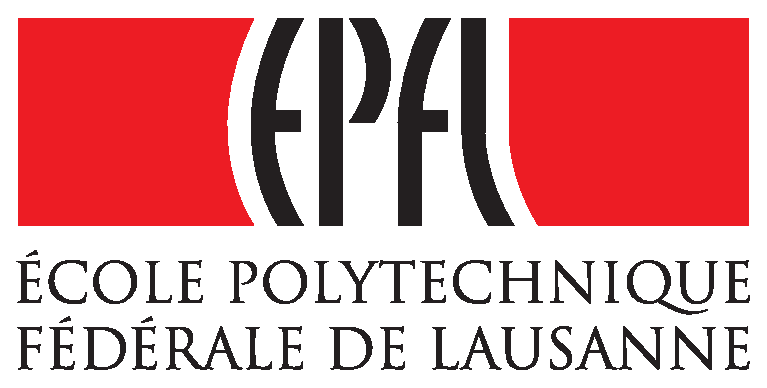
\includegraphics[width=4cm]{cover/logo_epfl_coul.eps}
  \end{center}
  \vspace{0.3cm}
  \hrule
}
\newcommand{\logolasec}[0]{
  \vspace{1cm}
  \hrule
  \begin{center}
    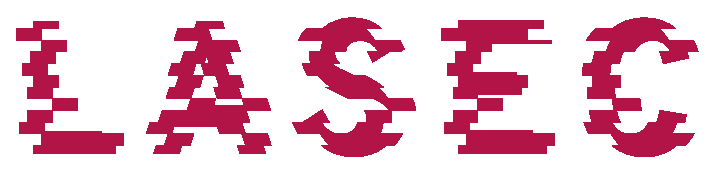
\includegraphics[width=4.5cm]{cover/logo_lasec_coul.eps}
  \end{center}
}
\newcommand{\project}[1]{
  \begin{center}
    \large{#1}
  \end{center}
  \vspace{1cm}
}
\newcommand{\department}[1]{
  \begin{center}
    \large{#1}
  \end{center}
}
\newcommand{\supervisor}[3]{
  \begin{center}
    \begin{normalsize}{
        \bfseries #1}\\#2\\#3
    \end{normalsize}
  \end{center}
}
\renewcommand{\author}[1]{
  \begin{center}
    \Large{#1}
  \end{center}
  \vspace{0.5cm}
}
\renewcommand{\title}[1]{
  \vspace{3cm}
  \begin{center}
    \huge{#1}
  \end{center}
  \vspace{1.7cm}
}
\renewcommand{\date}[2]{
  \begin{center}
    \normalsize{#1 #2}
  \end{center}
  \vspace{0.5cm}
}


\thispagestyle{empty}


% begin title page
\logoepfl

\title{Ratcheting}

\author{Andrea Caforio}
\department{School of Computer and Communication Sciences}
\project{Optional Semester Project}

\date{January}{2019}

\begin{center}
  \begin{tabular}{cc}
    \begin{tabular}{p{4.0cm}}
      \supervisor{Responsible}{Prof. Serge Vaudenay}{EPFL / LASEC}
    \end{tabular}&
    \begin{tabular}{p{4.0cm}}
      \supervisor{Supervisor}{Dr. Betül Durak}{EPFL / LASEC}
    \end{tabular}
  \end{tabular}
\end{center}

\logolasec
% end title page




% Updated March 2006 (SP)


\newcommand{\logoepfl}[0]{
  \begin{center}
    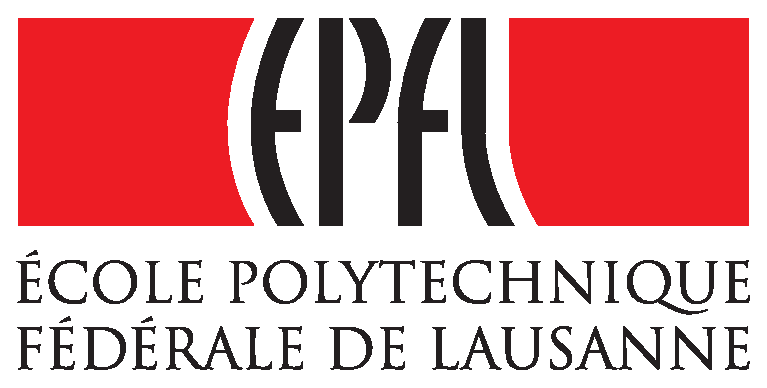
\includegraphics[width=4cm]{cover/logo_epfl_coul.eps}
  \end{center}
  \vspace{0.3cm}
  \hrule
}
\newcommand{\logolasec}[0]{
  \vspace{1cm}
  \hrule
  \begin{center}
    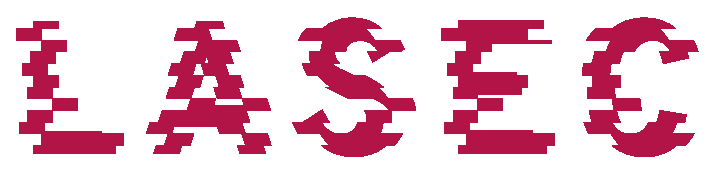
\includegraphics[width=4.5cm]{cover/logo_lasec_coul.eps}
  \end{center}
}
\newcommand{\project}[1]{
  \begin{center}
    \large{#1}
  \end{center}
  \vspace{1cm}
}
\newcommand{\department}[1]{
  \begin{center}
    \large{#1}
  \end{center}
}
\newcommand{\supervisor}[3]{
  \begin{center}
    \begin{normalsize}{
        \bfseries #1}\\#2\\#3
    \end{normalsize}
  \end{center}
}
\renewcommand{\author}[1]{
  \begin{center}
    \Large{#1}
  \end{center}
  \vspace{0.5cm}
}
\renewcommand{\title}[1]{
  \vspace{3cm}
  \begin{center}
    \huge{#1}
  \end{center}
  \vspace{1.7cm}
}
\renewcommand{\date}[2]{
  \begin{center}
    \normalsize{#1 #2}
  \end{center}
  \vspace{0.5cm}
}


\thispagestyle{empty}


% begin title page
\logoepfl

\title{Ratcheting}

\author{Andrea Caforio}
\department{School of Computer and Communication Sciences}
\project{Optional Semester Project}

\date{January}{2019}

\begin{center}
  \begin{tabular}{cc}
    \begin{tabular}{p{4.0cm}}
      \supervisor{Responsible}{Prof. Serge Vaudenay}{EPFL / LASEC}
    \end{tabular}&
    \begin{tabular}{p{4.0cm}}
      \supervisor{Supervisor}{Dr. Betül Durak}{EPFL / LASEC}
    \end{tabular}
  \end{tabular}
\end{center}

\logolasec
% end title page




% Updated March 2006 (SP)


\newcommand{\logoepfl}[0]{
  \begin{center}
    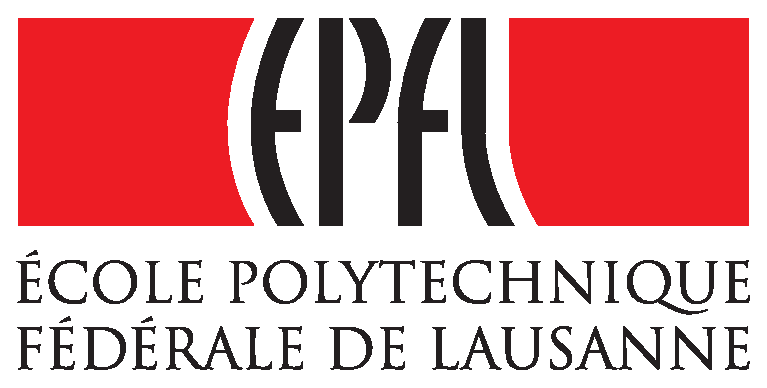
\includegraphics[width=4cm]{cover/logo_epfl_coul.eps}
  \end{center}
  \vspace{0.3cm}
  \hrule
}
\newcommand{\logolasec}[0]{
  \vspace{1cm}
  \hrule
  \begin{center}
    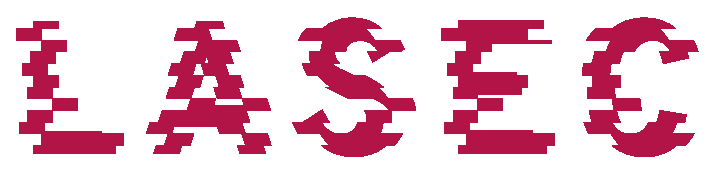
\includegraphics[width=4.5cm]{cover/logo_lasec_coul.eps}
  \end{center}
}
\newcommand{\project}[1]{
  \begin{center}
    \large{#1}
  \end{center}
  \vspace{1cm}
}
\newcommand{\department}[1]{
  \begin{center}
    \large{#1}
  \end{center}
}
\newcommand{\supervisor}[3]{
  \begin{center}
    \begin{normalsize}{
        \bfseries #1}\\#2\\#3
    \end{normalsize}
  \end{center}
}
\renewcommand{\author}[1]{
  \begin{center}
    \Large{#1}
  \end{center}
  \vspace{0.5cm}
}
\renewcommand{\title}[1]{
  \vspace{3cm}
  \begin{center}
    \huge{#1}
  \end{center}
  \vspace{1.7cm}
}
\renewcommand{\date}[2]{
  \begin{center}
    \normalsize{#1 #2}
  \end{center}
  \vspace{0.5cm}
}


\thispagestyle{empty}


% begin title page
\logoepfl

\title{Ratcheting}

\author{Andrea Caforio}
\department{School of Computer and Communication Sciences}
\project{Optional Semester Project}

\date{January}{2019}

\begin{center}
  \begin{tabular}{cc}
    \begin{tabular}{p{4.0cm}}
      \supervisor{Responsible}{Prof. Serge Vaudenay}{EPFL / LASEC}
    \end{tabular}&
    \begin{tabular}{p{4.0cm}}
      \supervisor{Supervisor}{Dr. Betül Durak}{EPFL / LASEC}
    \end{tabular}
  \end{tabular}
\end{center}

\logolasec
% end title page


\tableofcontents

\chapter{Introduction}
\label{chap:introduction}

Messaging has become an ubiquitous resource in the daily lives of
millions of people around the globe through the widespread adoption of
instant messaging applications. The design of protocols which
facilitate securing messaging or key-agreement is faced with a unique
set of challenges, this is due to the longevity of sessions between
communicating parties and the inherently asynchronous notion of
messaging where a participant is both the sender and recipient of
messages and the time a message is sent or received is undefined. In
such a setting the leakage of a state to the adversary is especially
devastating since in a naive protocol it would not only enable him to
recover past messages but also allow decryption of future messages as
well as impersonations of the victim.
% \begin{figure}[h]
\begin{wrapfigure}{r}{0.46\textwidth}
  \centering
  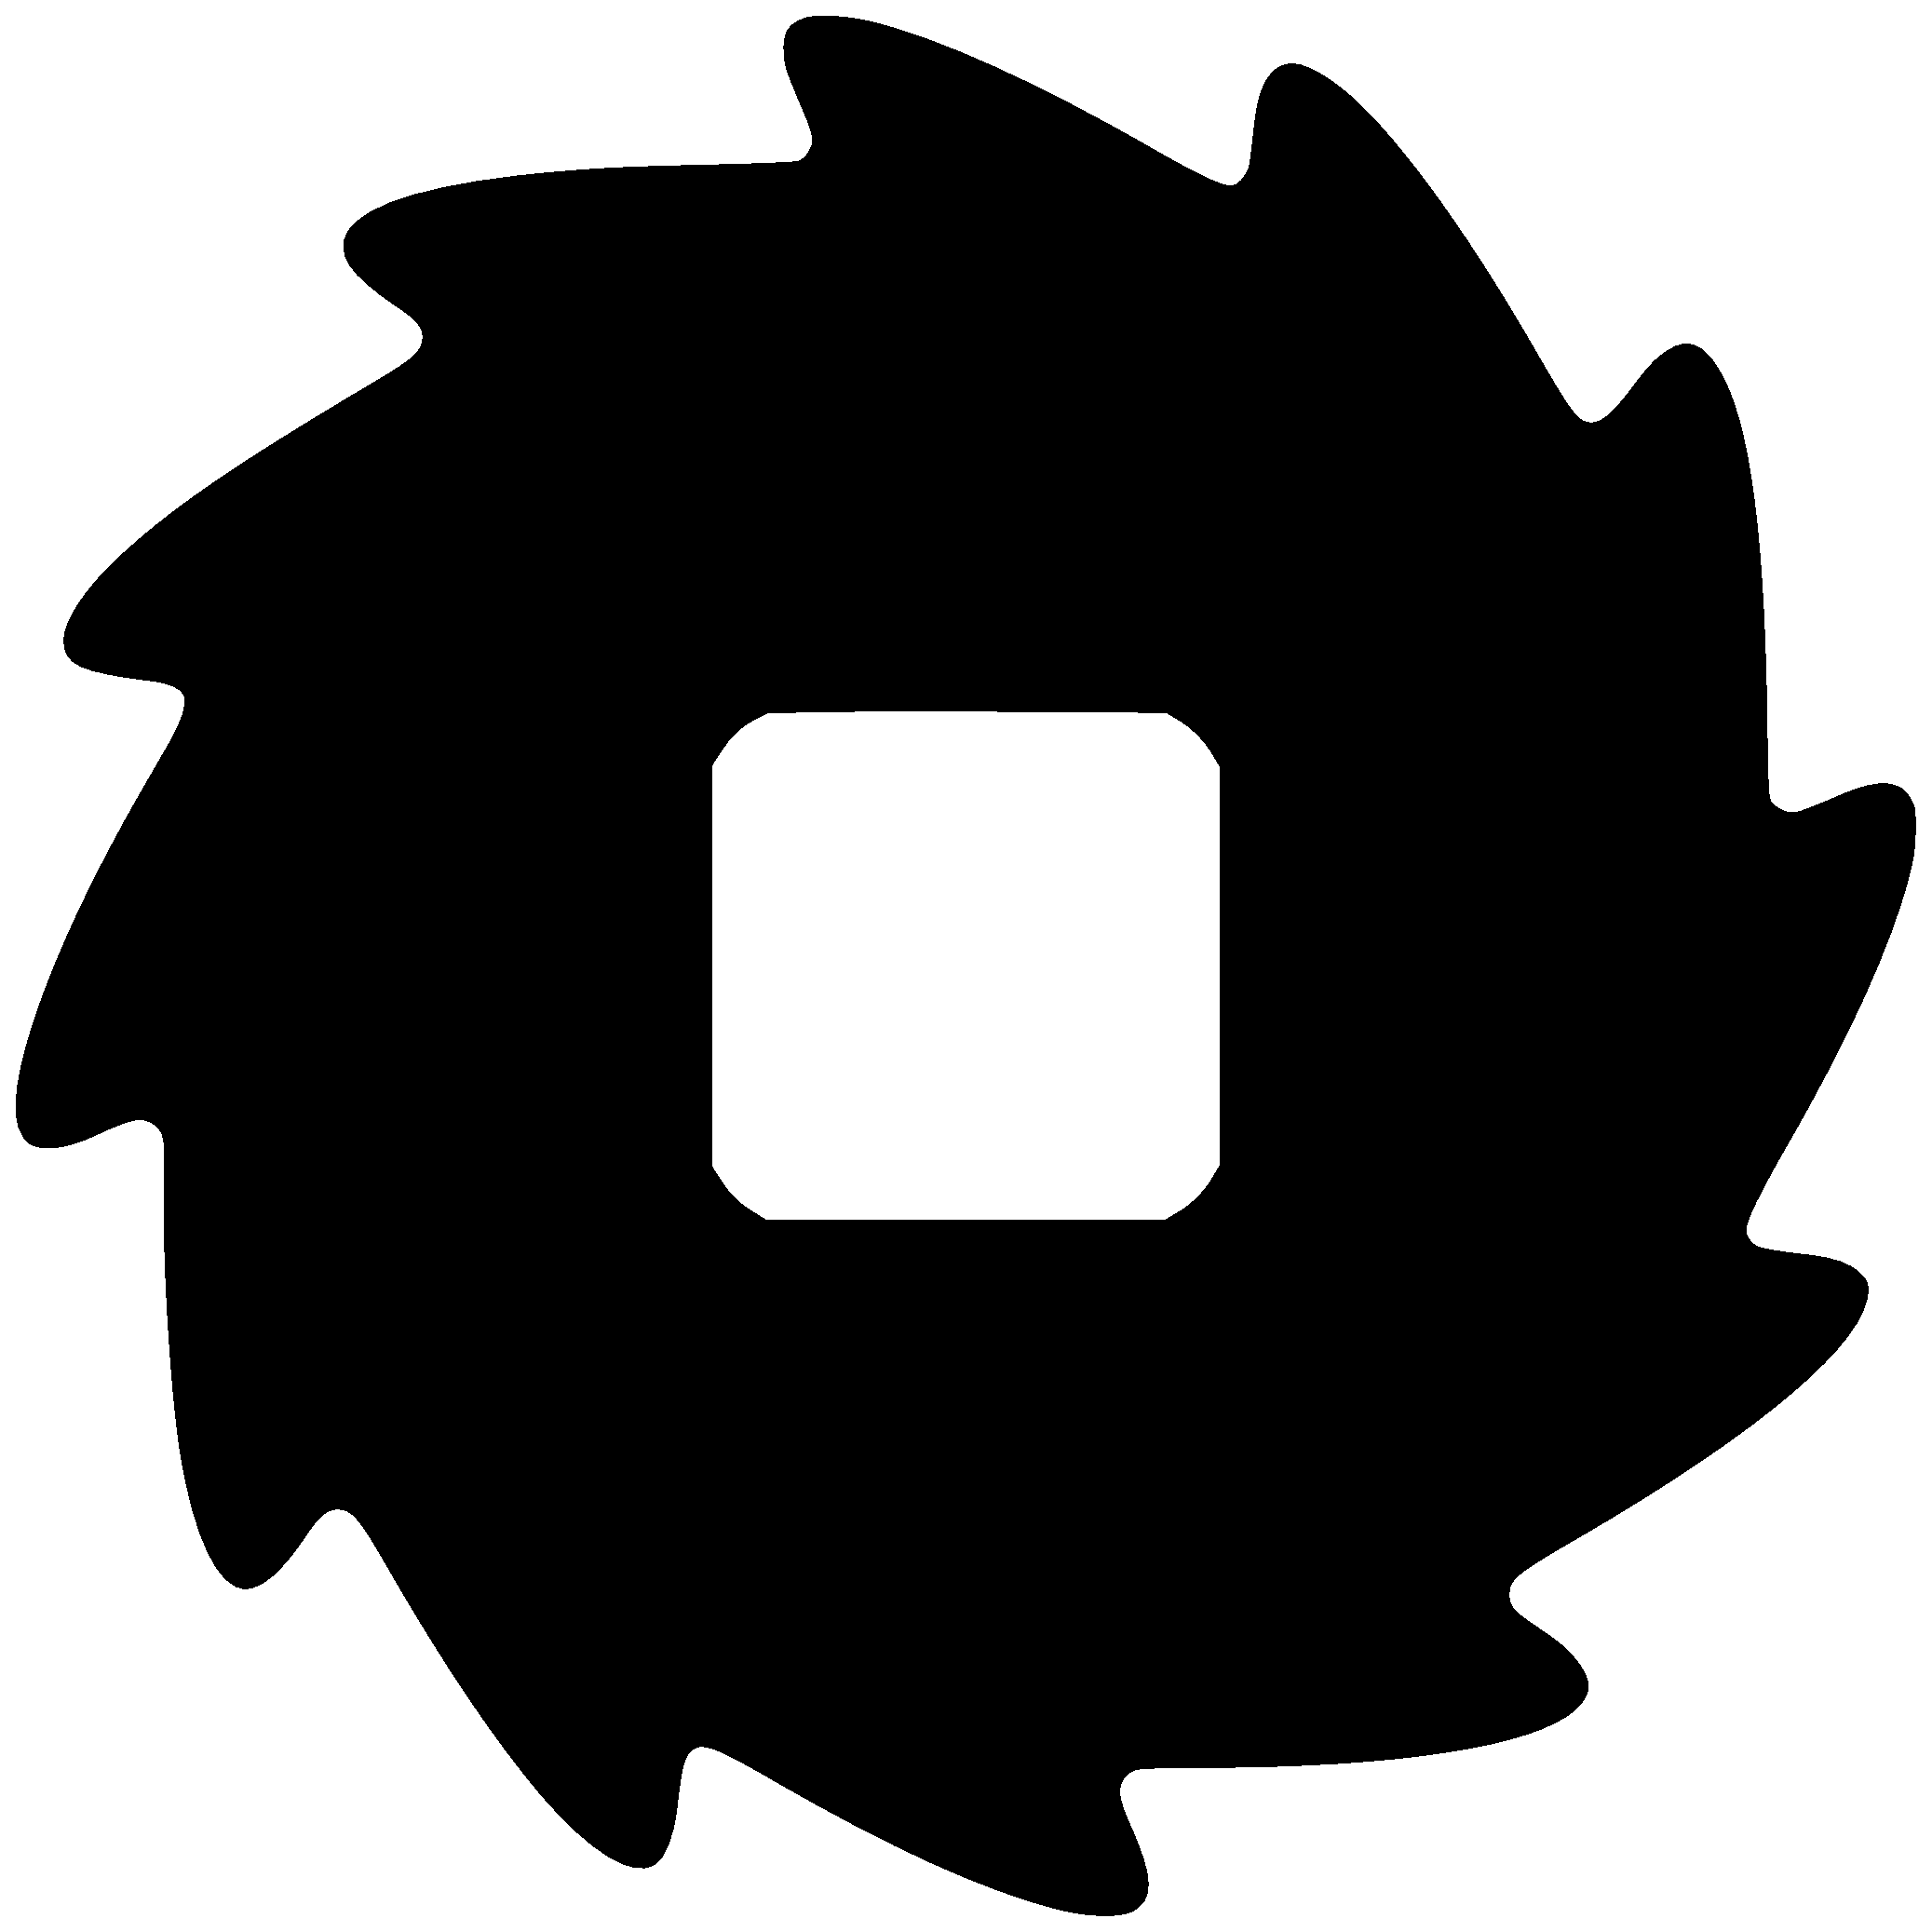
\includegraphics[width=0.42\textwidth]{figures/ratchet-icon.eps}
  \caption[Symbolic Ratchet Wheel]{Symbolic Ratchet Wheel\footnotemark}
  \label{fig:ratchet-wheel}
  % \end{figure}
\end{wrapfigure}
\footnotetext{\url{https://www.iconfinder.com/icons/328526}} Ratcheting has
established itself as the go-to technique in
order to mitigate these risks. Akin to its mechanical equivalent the
user states are continuously moved forward (updated) without the
possibility of going backwards, i.e.~it should be impossible to
recover past states from the current one.
This further implies that
past messages remain secure even in the presence of an adversary who
can expose the state of a participant. The literature labels protocols
that deploy ratchets as \textit{forward-secure}. This technique saw
its inception in 2004 as part of the Off-the-Record messaging
protocol~\cite{borisov2004off}. It only recently gained traction
through the massively popular Signal protocol~\cite{perrin2016double}.
The release of this protocol however predates its first formal
security analysis in 2017~\cite{cohn2017formal}
and since then several novel protocols with various degrees of
security guarantees have been proposed. Among others
these protocols also attempt the satisfy the notion of
\textit{future secrecy} or post-compromise security in which future states and
messages remain secure after a state exposure. Furthermore, a secure messaging
protocol should be efficient enough to run smoothly even on
computationally inferior devices thus the choice of fast primitives
that do not compromise the promised security levels play a crucial
part in the construction of messaging protocols. Even though on paper
the attained levels of security in these new protocol often only
differ marginally the effects on performance metrics are of a
different kind with sometimes huge differences between the protocols.
%
%\section{Contributions}
%\label{sec:contributions}
%
This project is concerned with surveying and solidifying the
performance differences of seven new secure messaging or key-agreement
protocols that have been proposed throughout 2018. In
chapter~\ref{chap:protocols} the notion of secure messaging and
especially ratcheting is briefly reviewed before each protocol is
summarized in terms of composition, primitives and security levels, then in
chapter~\ref{chap:benchmarks} the protocols are measured and compared
on the basis of several benchmarks. The report is then concluded
in the last chapter with some general remarks.
%
%\section{Circumstances}
%\label{sec:circumstances}
%

\bigskip

This project has been conducted as part of the third master semester optional
semester project in computer science course (CS-596) offered by the
School of Computer and Communications Sciences at EPFL and is credited
with eight points. It was supervised by Doctor Betül Durak of
the LASEC laboratory.

\chapter{Protocols}
\label{chap:protocols}

As laid out in the introduction the Signal~\cite{perrin2016double}
protocol was created and deployed well before the establishment of a
serious secure messaging definition thus it was lacking any form of
formal security proof. The subsequent analysis in 2017~\cite{cohn2017formal}
was then more concerned with proving the security of specific Signal
instances than treating the general case of secure
messaging. Formally, ratcheted messaging attempts to satisfy some
correctness and security notions.

\section{Ratcheted Messaging}
\label{sec:ratcheted-messaging}

For the remainder of this text let Alice and Bob be the communicating
parties exchanging messages through an insecure channel. Alice and Bob take on random
roles throughout their communication and are not necessarily
synchronized meaning that the reception of sent messages may be
delayed to a point where there are already new messages in the channel
travelling in the opposite direction. Note that this does not imply
that messages may be dropped or received in a different order than
they were initially sent in, this will be important later on when
the actual protocols are described.
\begin{figure}[ht]
  \centering
  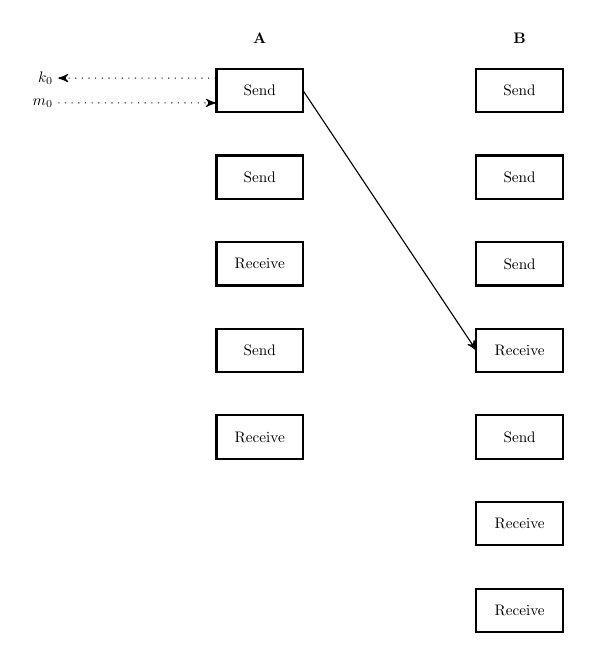
\begin{tikzpicture}[
  box/.style={rectangle,draw,inner sep=5pt,minimum height=1cm,minimum width=2cm,thick},
  node distance=2cm,
  ->,>=stealth',
  scale=0.55, every node/.style={scale=0.55}
]

  % Box t0
  \node [box] (t0) {Send};
  \node [coordinate,right of=t0,node distance=1cm] (tl0) {};
  \node [coordinate,above left=-0.125cm and 0cm of t0,node distance=1cm] (ta0) {};
  \node [left=2cm of ta0] (taa0) {$k_0$};
  \path (ta0) edge[dotted] node [] {} (taa0);
  \node [coordinate,below left=-0.125cm and 0cm of t0,node distance=1cm] (tb0) {};
  \node [left=2cm of tb0] (tbb0) {$m_0$};
  \path (tbb0) edge[dotted] node [] {} (tb0);


  \node [box,below of=t0] (t1) {Send};
  \node [box,below of=t1] (t2) {Receive};
  \node [box,below of=t2] (t3) {Send};
  \node [box,below of=t3] (t4) {Receive};

  \node [box,right of=t0,node distance=6cm] (t5) {Send};
  \node [box,below of=t5] (t6) {Send};
  \node [box,below of=t6] (t7) {Send};
  \node [box,below of=t7] (t8) {Receive};
  \node [box,below of=t8] (t9) {Send};
  \node [box,below of=t9] (t10) {Receive};
  \node [box,below of=t10] (t11) {Receive};

  \node [coordinate,left of=t8,node distance=1cm] (tl8) {};
  \path (tl0) edge[] node [] {} (tl8);

  \node [above=0.25cm of t0] (alice) {\bfseries{A}};
  \node [above=0.25cm of t5] (bob) {\bfseries{B}};
\end{tikzpicture} 
  \caption{Example of Ratcheted Traffic}
  \label{fig:traffic}
\end{figure}
Figure~\ref{fig:traffic} shows an example asynchronous traffic
transcript for both messaging and key-agreement. The initial states of
Alice and Bob are created and distributed by a trusted party, these
states are updated with each send or receive operation. In the case of
a key-agreement protocol the update information corresponding to the
created key of the sender should generate the same key at the receiver
when the update message is received. Analogous, for a messaging
protocol where an encrypted message should be correctly deciphered by
the receiver upon arrival. In figure~\ref{fig:traffic} for example,
the message sent by Alice at time $t_0$ is only received by Bob at
time $t_8$ but should nonetheless produce a correct key or plaintext
regardless of the messages sent by Bob in the meantime that have
updated Bob's state.

\section{Ratchet Security}
\label{sec:ratchet-security}

These continuous updates of the states are supposed to be irreversible
such that past states may not be derived from any future state thus
yielding forward security which in turn protects past messages from being
compromised. This was the original goal that ratcheting tried to
achieve. Naively, a ratchet can be constructed through the usage of a
one-way function the simply updates the states of the communicating
parties. In practice, a hash-function would be deployed as a
reasonable alternative with the downside of losing the asynchronous
communication property~\cite{bellare2003forward}. On the other hand if
some randomness is included in the creation of an updated state we can
protect future states from being recreated by an adversary after an
exposure yielding future secrecy or post-compromise security. Another
way is the usage of some key-agreement protocol to schedule the
creation of new states between the parties~\cite{cohn2016post}. Again
both constructions come at the cost of losing asynchronous
communications. Asynchronous communications is thus a challenging
obstacle that significantly complicates the design and analysis
of ratcheted key-agreement or messaging protocols.

\bigskip

The adversary in ratcheted protocols is quite powerful and can be both
passive and to a certain extend active. This means he has access to
the full message transcript, can expose the states of both
participants and corrupt the states. As it is
usual in such cases we assess the advantage of any adversary as part
of some key indistinguishability (KIND) or ciphertext (CIND)
indistinguishability game where the adversarial algorithm $\mathcal{A}$
has access to the send and receive procedures of both Alice and Bob can expose their states
and in the end tries to distinguish between some key or a uniformly
random source string in the KIND
game or decide which one of two chosen messages corresponds to a given
ciphertext in the CIND game.
Figure~\ref{fig:kind} depicts a generic KIND game where \texttt{RATCH} denotes
the send or receive procedures for both Alice and Bob, at will callable by the
adversary. We can similarly define the CIND game in figure~\ref{fig:cind}.
It is important to note that the way the games are defined is
not sufficient since there exist trivial strategies that make an adversary
succeed. If for example Bob's state is exposed right before he
receives a message then an adversary can easily recover the plaintext
from the message in a messaging protocol or compute the session key
from the message in a key-agreement protocol. It is exactly the
identification of such attacks that pose the greatest
challenge in the analysis of ratcheted protocols implying that the security games
have to be modified to disallow these trivial attacks. Naturally,
the fewer attacks are excluded by the games the securer the overall
protocol becomes. Once the games have been adjusted we can
quantify the advantage of any algorithm restricted to some number of queries
and some time complexity as
\[
  \t{Adv}(\mathcal{A}) = \left| \Pr \left[ \t{\{C,K\}IND}_0^\mathcal{A} \rightarrow 1 \right] -
                                \Pr \left[ \t{\{C,K\}IND}_1^\mathcal{A} \rightarrow 1 \right]
                         \right|.
\]

\begin{figure}[ht]
  \centering
  \setlength{\fboxsep}{10pt}
  \scalebox{0.9}{%
    \fbox{%
       \algrenewcommand\textproc{}
 \algrenewcommand\algorithmicprocedure{\textbf{Game}}

 \begin{minipage}{.5\linewidth}
   \begin{algorithmic}[1]
     \Procedure{$\t{KIND}_b^\mathcal{A}$}{}
     \State $(\t{st}_\t{A},\t{st}_\t{B}) \gets$ \Call{Init}{$1^\lambda$}
     \State $b' \gets \mathcal{A}^{\t{RATCH,EXP,TEST}}$
     \State \Return $b'$
     \EndProcedure
   \end{algorithmic}
 \end{minipage}

 \vline

 \algrenewcommand\textproc{}
 \algrenewcommand\algorithmicprocedure{\textbf{Oracle}}

 \begin{minipage}{.5\linewidth}
   \begin{algorithmic}[1]
     \Procedure{TEST}{$\t{P}$}
     \If{$b = 1$}
     \State \Return $k_\t{P}$
     \EndIf
     \State \Return random $\{0,1\}^{|k_\t{P}|}$ 
     \EndProcedure

     \item[] % Blank line.

     \Procedure{EXP}{$\t{P}$}
     \State \Return $\t{st}_\t{P}$ 
     \EndProcedure
  \end{algorithmic}
\end{minipage}%

    }
  }
  \caption{Generic Key-Indistinguishability Game}
  \label{fig:kind}
\end{figure}

\begin{figure}[ht]
  \centering
  \setlength{\fboxsep}{10pt}
  \scalebox{0.9}{%
    \fbox{%
      \algrenewcommand\textproc{}
  \algrenewcommand\algorithmicprocedure{\textbf{Game}}

  \begin{minipage}{.5\linewidth}
    \begin{algorithmic}[1]
      \Procedure{$\t{CIND}_b^\mathcal{A}$}{}
      \State $(\t{st}_\t{A},\t{st}_\t{B}) \gets$ \Call{Init}{$1^\lambda$}
      \State $b' \gets \mathcal{A}^{\t{RATCH',EXP}}$
      \State \Return $b'$
      \EndProcedure
    \end{algorithmic}
  \end{minipage}

  \vline

  \algrenewcommand\textproc{}
  \algrenewcommand\algorithmicprocedure{\textbf{Oracle}}

  \begin{minipage}{.5\linewidth}
    \begin{algorithmic}[1]
      \Procedure{RATCH'}{$\t{P},m_0,m_1$}
      \State \Return \Call{RATCH}{$\t{P},m_b$}
      \EndProcedure

      \item[] % Blank line.

      \Procedure{EXP}{$\t{P}$}
      \State \Return $\t{st}_\t{P}$ 
      \EndProcedure
   \end{algorithmic}
 \end{minipage}%

    }
  }
  \caption{Generic Ciphertext-Indistinguishability Game}
  \label{fig:cind}
\end{figure}

\section{A Brief History of Ratcheted Protocols}
\label{sec:brief-hist-ratch}

As already pointed out the formal analysis of Signal in 2017 marked the
starting point for a slew of ratcheted messaging and key-agreement
protocols. The first protocol was proposed by Bellare et
al.~\cite{bellare2017ratcheted} which established a secure key
exchange protocol for the unidirectional channel that however does not
permit any exposures of the receiver state. Afterwards, Poettering and
Rösler~\cite{poettering2018towards} presented a secure bidirectional
key-agreement protocol in the random oracle model. Around the same
time Jaeger and Stepanovs~\cite{jaeger2018optimal} proposed a
messaging protocol targeting the same security level deploying
similar cryptographic primitives. To this date, these two protocols achieve the
highest degree of security at the cost of extremely increased running
times. Later on Durak and Vaudenay~\cite{durak2018bidirectional}
published an efficient bidirectional key-agreement protocol with minor
concessions in terms of security compared to
\cite{poettering2018towards} and \cite{jaeger2018optimal}. Next in
the line was a messaging protocol by Jost, Maurer and
Mularczyk~\cite{jostefficient} attempting to close the gap between
\cite{durak2018bidirectional} and
\cite{poettering2018towards,jaeger2018optimal}. It offers a higher
security level than \cite{durak2018bidirectional}, though not reaching
\cite{poettering2018towards,jaeger2018optimal}, but is slower in
comparison. The currently last protocol in the line is a secure messaging construction
from Alwen, Coretti, and Dodis~\cite{alwen2018double}. It takes
a different approach than the other protocols by building an
improved version of the original Signal protocol instead of
coming up with an entirely new protocol. It is an efficient protocol
that does not quite hold up with the other protocols in terms of
security but is the only one that offers \textit{immediate decryption},
the ability to decipher messages even if messages are lost or arrive in
a different order that than they were initially sent in.
In the following sections we will look more closely into all
above described protocols, except~\cite{bellare2017ratcheted}.

\section{Notation}
\label{sec:notation}

All the protocols depicted in the following figures are as closely
as possible depicted in respect to the original prints in their respective
papers only omitting lines that are not necessary
to understand the benchmark results. The pseudo-code should be self-contained
but there are nonetheless
some special symbols. We let $\perp$ denote the \texttt{null} symbol.
$||$ represents the concatenation of two byte strings. An empty
array is described by $[\cdot]$. Ellipses in the array selector
$A[...,i]$ are used to
denote an operation on multiple array elements and last but not least
$\leftarrow$ is the assignment operator.

\section[BARK (Poettering and Rösler)]
{BRKE (Poettering and Rösler)~\cite{poettering2018towards}}
\label{sec:poettering-roesler}

This asynchronous key-agreement protocol was released in the paper
\textit{Asynchronous Ratcheted Key Exchange} in May 2018.
The fact that sets this protocol, and the protocol in the following
section, apart from the others is the notion of post-impersonation security
also called fine-grained post-compromise security,
meaning that there still remain some security guarantees concerning
messages that follow a successful
impersonation attempt. Post-impersonation security can be further divided
into authenticity and confidentiality.
\begin{itemize}
\item \textbf{Post-Impersonation Authentication.} Assume the adversary
  managed to inject a message to Bob effectively impersonating Alice.
  Post-impersonation authenticity makes sure that any further message
  from Bob or the adversary will be rejected by Alice. This should even hold if
  Bob's state is compromised after the injection. Chain-hashing
  the communication transcript is a simple way to reject messages from
  Bob after an injection for the case where Bob's state has not
  been compromised. As we will see in section~\ref{sec:durak-vaudenay}
  a similar notion called recover security is one of the corner stones
  of the protocol by Durak and Vaudenay. However, maintaining authenticity
  after an injection with an additional state leakage is another level
  and seems to require heavy primitives as deployed in this protocol.
\item \textbf{Post-Impersonation Confidentiality.} Again assume
  that the adversary managed to have an injected message accepted by Bob,
  post-impersonation confidentiality ensures that future messages from
  Alice to Bob remain
  confidential even if Bob's state is exposed after the injection.
\end{itemize}
In section~\ref{sec:jost-maur-mularczyk} we will see a protocol
that comes close to providing full post-impersonation security
if some additional properties are satisfied while only relying on
public-key cryptography instead of the extremely inefficient
primitives in this and the following protocol. It is conjectured
that the security level achieved by BRKE and the protocol
in the next section is optimal, setting the upper-bound
on what a ratcheted protocol can reach.

\subsection{Primitives}
\label{sec:primitives}

The protocol proposes a new cryptographic primitive that extends the
functionality of an ordinary key-encapsulation mechanism with
key update algorithms and is the principal tool with whom the
protocol achieves forward and future secrecy as well as
post-impersonation resilience.
\begin{itemize}
\item \textbf{Key-Updatable Key-Encapsulation Mechanism (ku-KEM).} The primitive
  consists of four procedures, a initial key generation algorithm \texttt{Gen}, an
  key-encapsulation procedure \texttt{Enc}, a corresponding decapsulation
  procedure \texttt{Dec} and
  update procedures for both the public \texttt{UpdPk} and secret key \texttt{UpdSk}.
  \begin{align*}
    \texttt{Gen} & : \ \rightarrow \mathcal{SK} \times \mathcal{VK} \\
    \texttt{Enc} & : \mathcal{PK} \rightarrow \mathcal{K} \times \mathcal{C} \\ 
    \texttt{Dec} & : \mathcal{SK} \times \mathcal{C} \rightarrow \mathcal{K} \\
    \texttt{UpdPk} & : \mathcal{PK} \times \Delta \rightarrow \mathcal{PK} \\
    \texttt{UpdSk} & : \mathcal{SK} \times \Delta \rightarrow \mathcal{SK}
  \end{align*}
  $\mathcal{PK}$ is the public key domain, $\mathcal{SK}$ is the secret key domain,
  $\mathcal{AD}$ is the associated data domain and $\Delta$ is
  the update information domain.
\end{itemize}
In security terms a ku-KEM should satisfy the guarantees of regular
key-encapsulation mechanisms in addition to forward security that
protecting past keys from state exposures. A ku-KEM can be generically constructed
out of any hierarchical identity-based encryption scheme
(HIBE)~\cite{gentry2002hierarchical}. Contrary to an ordinary
identity-based encryption scheme where there is a single central
authority handing out secret keys to the users, a HIBE consists
of hierarchical tree structure of many authorities on different levels
such that an authority can distribute keys to its children authorities.
More formally a HIBE scheme consists of four routines, a setup
function that generates the public parameters and the secret key
of the root authority, an extraction function where a parent creates
a secret key for one of its children, an encryption
function that enciphers a message for a given identity and
its corresponding decryption function recovering the message.
An authority has the ability to decrypt all ciphertexts
encrypted by its descendants but not those by its ancestors.
Is then not hard to see that key extractions in a HIBE
can be used to provide key update functionalities to
a surrounding primitive as it is the case in the ku-KEM.
Naturally, the deeper the hierarchy the larger become the
created keys slowing down the encryption and decryption procedures.
As with ordinary identity-based encryption schemes HIBE schemes are usually
pairing- or lattice-based which is far more inefficient,
than performing operations over for example elliptic curves.
There is also a lack of hardened pairing- or lattice-based
cryptography libraries making ku-KEM harder to actually
implement.
Next to a HIBE construction, the protocol further needs a regular digital
signature scheme DS (\texttt{Gen,Sign,Verify}) and a random oracle \texttt{H}.

\subsection{Construction}
\label{sec:construction}

Poettering and Rösler give three separate constructions in their article.
A unidirectional protocol (URKE), a sesquidirectional construction (SRKE) in which
Bob can reply without actually establishing session keys, finally both URKE and SRKE
are used to create a bidirectional asynchronous key-exchange protocol (BRKE)
with optimal security. The construction is quite involved with long
procedures, figure~\ref{fig:brke} prunes out some parts not necessary for the
analysis of the benchmarks in the next chapter. The protocol proceeds
in epochs indicated by the $(E_S^\vdash,E_S^\dashv)$ and $(E_R^\vdash,E_R^\dashv)$
variables that steer the creation of encapsulations and key updates.
Prolonged periods of unidirectional traffic will enlarge the
difference between $(E_R^\vdash,E_R^\dashv)$ for the sending
party and $(E_S^\vdash,E_S^\dashv)$ for the receiving party.
In other words the participants are constantly exchanging
ku-KEM and Signature keys. If some messages are delayed such
that a participant receives a message from a previous epoch
then both users will perform key-updates to ensure forward-security.

\begin{itemize}
\item \textbf{Init.} Two sets of ku-KEM, DS and hashing keys are generated
  and distributed to the participants. Furthermore, each user has a counter
  for sent messages $s$ and for received messages $r$ next to the epoch
  counters unified under the variable $E$. The accumulated ku-KEM keys
  are stored in the arrays (SK,PK) with $(L_S,L_R,t)$ storing the transcript
  of sent and received messages.
\item \textbf{Send}. Each send operation generates a new set of
  ku-KEM and DS keys where the encapsulation key $pk^*$ and the
  signature verification key $sk^*$ are sent along the ciphertext
  together with a signature $\sigma$ and the current $E_S^\dashv$ epoch
  counter. The users will
  accumulate the created ku-KEM keys and when the direction
  of traffic changes after a period of unidirectional communication
  they will use all the accumulated keys to establish the new
  session key before deleting the accumulated ku-KEM public keys.
  Further note that the
  session key is derived by using the ku-KEM encapsulation data
  as input to the random oracle.
\item \textbf{Receive.} The receive operation mirrors the
  operations in the send function. With the addition
  of updating the ku-KEM keys in case the epoch counters have diverged.
  Note that the protocol requires that the entire message protocol
  is stored within $t_S$ which simplifies some of the security
  proofs provided in~\cite{poettering2018towards} meaning that
  the user states are growing as time progresses. Also note
  that each key update in a loop is equivalent to deepening
  the HIBE hierarchy within the ku-KEM making an unbounded
  hierarchy necessary.
\end{itemize}

\begin{figure}[p]
  \centering
  \setlength{\fboxsep}{10pt}
  \scalebox{0.9}{%
    \fbox{%
      \algrenewcommand\textproc{}
\algrenewcommand\algorithmicprocedure{\textbf{func}}

\begin{minipage}{0.5\linewidth}
  {\fontsize{8}{10}\selectfont

  \begin{algorithmic}[1]
    \Procedure{Init}{$K_\t{A},K_\t{B}$}
    \For{$u \in \{A,B\}$}
    \State $(sgk_\t{u},vfk_\t{u}) \gets$ \Call{DS.Gen}{}
    \State $(sk_\t{u},pk_\t{u}) \gets$ \Call{KEM.Gen}{}
    \State $E^\vdash \gets 0, \ E^\dashv \gets 0$
    \State $s \gets 0, \ r \gets 0, \ t \gets \perp$
    \State $PK_\t{u}[0] \gets pk, \ SK_\t{u}[0] \gets sk$
    \State $L_\t{S}[0] \gets \perp, \ L_\t{R}[0] \gets \perp$
    \State $S_\t{u} \gets (PK_{\bar{\t{u}}},E,s,L_\t{S},
                          vfk_{\bar{\t{u}}},K_{\bar{\t{u}}},t)$
    \State $R_\t{u} \gets (SK_\t{u},E,r,L_\t{R},sgk_\t{u},K_\t{u},t)$
    \State $ST_\t{u} \gets (S_\t{u},R_\t{u})$
    \EndFor
    \State \Return $(ST_\t{A},ST_\t{B})$
    \EndProcedure
    
    \item[]
    
    \Procedure{Send}{$ST, ad$}
    \State $(\sigma_\t{root},v,\gamma,T_\t{cur},t_\t{A}) \gets \t{st}_\t{A}$
    \State $(R,S) \gets ST$
    \State $(SK,E_\t{R},r,L_\t{R},sgk,K_\t{R},t_\t{R}) \gets R$
    \State $(sgk^*,vfk^*) \gets$ \Call{DS.Gen}{}
    \State $(sk^*,pk^*) \gets$ \Call{DS.Gen}{}
    \State $E_\t{R}^\vdash \gets E_\t{R}^\vdash+1, \ SK[E_\t{R}^\vdash] \gets sk^*$
    \State $C \gets r || pk^* || vfk^*$
    \State $(PK,E_\t{S},s,L_\t{S},vfk,K_\t{S},t_\t{S}) \gets S$
    \State $k^* \gets \perp, \ C \gets C || E_\t{S}^\dashv$
    \For{$e' \gets E_\t{S}^\vdash$ to $E_\t{S}^\dashv$}
    \State $(k,c) \gets$ \Call{KEM.Enc}{$PK[e']$}
    \State $k^* \gets k^* || k, \ C \gets C || c$ 
    \EndFor
    \State $\sigma \gets$ \Call{sgn}{$sgk,ad||C$}
    \State $C \gets C || \sigma, \ L_\t{R}[E_\t{R}^\dashv] \gets ad||C$
    \State $R \gets (SK,E_\t{R},r,L_\t{R},sgk^*,K_\t{R},t_\t{R})$
    \State $t_\t{S} \gets ad||C$
    \State $k.o || K_\t{S} || k.m || sk \gets$ \Call{H}{$K_\t{S},k^*,L_\t{S}$}
    \State $pk \gets$ \Call{KEM.Gen}{$sk$}
    \State $PK[...,(E_\t{S}^\dashv -1)] \gets \perp, \ PK[E_\t{S}^\dashv] \gets pk$
    \State $E_\t{S}^\vdash \gets E_\t{S}^\dashv, \ s \gets s+1, \ L_\t{S}[s] \gets ad||C$
    \State $S \gets (PK,E_\t{S},s,L_\t{S},vfk,K_\t{S},t_\t{S})$
    \State $ST \gets (R,S)$
    \State \Return $(ST,k.o,C)$
    \EndProcedure
  \end{algorithmic}
  }
\end{minipage}
\begin{minipage}{0.5\linewidth}
  {\fontsize{8}{10}\selectfont

  \begin{algorithmic}[1]
    \Procedure{Recceive}{$ST,ad,C$}
    \State $(R,S) \gets ST$
    \State $(PK,E_\t{S},s,L_\t{S},vfk,K_\t{S},t_\t{S}) \gets S$
    \State $t^* \gets ad||C, \ t_\t{S} \gets t_\t{S} t^*, \ C || \sigma \gets C$
    \State \textbf{assert} \Call{DS.Verify}{$vfk,ad||C,\sigma$}
    \State $r||pk^*||vfk||C \gets C$
    \State $L\t{S}[...,(r-1)] \gets \perp$
    \For{$s' \gets r+1$  to $s$}
    \State $pk^* \gets$ \Call{KEM.UpdPk}{$pk^*,L\t{S}[s']$}
    \EndFor
    \State $E_\t{S}^\dashv \gets E_\t{S}^\dashv+1, \ PK[E_\t{S}^\dashv] \gets pk^*$
    \State $S \gets (PK,E_\t{S},s,L_\t{S},vfk,K_\t{S},t_\t{S})$
    \State $(SK,E_\t{R},r,L_\t{R},sgk,K_\t{R},t_\t{R}) \gets R$
    \State $k^* \gets \perp, \ e||C \gets C$
    \State $t_\t{R} \gets t_\t{R} || L_\t{R}[E_\t{R}^\vdash+1]||...||L_\t{R}[e]$
    \State $L_\t{R}[...,e] \gets \perp$
    \For{$e' \gets E_\t{R}^\vdash$ to $e$}
    \State $c||C \gets C$
    \State $k \gets$ \Call{KEM.Dec}{$SK[e'],c$}
    \State $k^* \gets k^* ||k$
    \EndFor
    \State $t_\t{R} \gets t_\t{R}||t^*$
    \State $k.o || K_\t{S} || k.m || sk \gets$ \Call{H}{$K_\t{R},k^*,L_\t{R}$}
    \State $SK[...,(e -1)] \gets \perp, \ SK[e] \gets sk$
    \For{$e' \gets e+1$  to $E_\t{R}^\dashv$}
    \State $SK[e'] \gets$ \Call{KEM.UpdSk}{$SK[e'],t^*$}
    \EndFor
    \State $E_\t{R}^\vdash \gets e, \ r \gets r+1$
    \State $R_\t{u} \gets (SK_\t{u},E,r,L_\t{R},sgk_\t{u},K_\t{u},t)$
    \State $ST \gets (R,S)$
    \State \Return $(ST,k.o)$ 
    \EndProcedure
  \end{algorithmic}
  }
\end{minipage}
    }
  }
  \caption{Bidirectional Asynchronous Key-Exchange Protocol (BRKE)}
  \label{fig:brke}
\end{figure}

\clearpage

\section[Secure Channel (Jaeger and Stepanovs)]
{Secure Channel (Jaeger and Stepanovs)~\cite{jaeger2018optimal}}
\label{sec:jaeger-stepanovs}

This secure messaging protocol was published in the paper
\textit{Optimal Channel Security Against Fine-Grained State Compromise: The Safety of Messaging}
in June 2018 and targets similar a security level as the protocol by
Poettering and Rösler although aiming at secure communication instead
of key-agreement. This means that the protocol also achieves
post-impersonation security at the cost of an increased running time due
to the usage of inefficient primitives. 

\subsection{Primitives}
\label{sec:primitives-1}

The protocol, again as in the Poettering and Rösler case, uses a HIBE to provide
key-update functionalities to an ordinary primitive.
\begin{itemize}
\item \textbf{Key-Updatable Public-Key Encryption Scheme (ku-PKE).} The primitive
  consists of five routines. A key generation algorithm \texttt{Gen},
  an encryption procedure \texttt{Enc}, a corresponding decryption
  function \texttt{Dec} and two update routines one for the
  encryption key \texttt{UpdEk} and one for the decryption key \texttt{UpdDk}.
  \begin{align*}
    \texttt{Gen} & : \ \rightarrow \mathcal{DK} \times \mathcal{EK} \\
    \texttt{Enc} & : \mathcal{EK} \times \mathcal{M} \rightarrow \mathcal{C} \\
    \texttt{Dec} & : \mathcal{DK} \times \mathcal{C} \rightarrow \mathcal{M} \\
    \texttt{UpdEk} & : \mathcal{EK} \times \Delta \rightarrow \mathcal{EK} \\
    \texttt{UpdDk} & : \mathcal{DK} \times \Delta \rightarrow \mathcal{DK}
  \end{align*}
  $\mathcal{EK}$ denotes the encryption key domain, $\mathcal{DK}$ the
  decryption key domain, $\mathcal{M}, \mathcal{C}$ the message and
  ciphertext domain respectively and $\Delta$ is the update information domain.
\end{itemize}

The construction of a ku-PKE is trivially performed out of a HIBE where updating
the decryption key \texttt{UpdDk} is equivalent to extracting a fresh key from
a parent authority. Jaeger and Stepanovs define a second novel primitive for use
in the final protocol.
\begin{itemize}
\item \textbf{Key-Updatable Digital Signature Scheme (ku-DSS).} The primitive
  consists of five routines. A key generation algorithm
  \texttt{DS.Gen}, a signing routine \texttt{DS.Sign}, its corresponding
  verification function \texttt{DS.Verify} and two key update routines
  one for the signing key \texttt{DS.UpdSk} and one for the verification
  key \texttt{DS.UpdVk}.
  \begin{align*}
    \texttt{Gen} & \  \rightarrow \mathcal{SK} \times \mathcal{VK} \\
    \texttt{Sign} & : \mathcal{SK} \times \mathcal{M} \rightarrow \Sigma \\
    \texttt{Verify} & : \mathcal{VK} \times \mathcal{M} \times \Sigma \rightarrow \{0,1\} \\
    \texttt{UpdSk} & : \mathcal{SK} \times \Delta \rightarrow \mathcal{SK} \\
    \texttt{UpdVk} & : \mathcal{VK} \times \Delta \rightarrow \mathcal{VK}
  \end{align*}
  $\mathcal{VK}$ is the signing key domain, $\mathcal{SK}$ the verification key
  domain, $\mathcal{M}, \Sigma$ are the message and signature domains and
  $\Delta$ is the update information domain.
\end{itemize}

A forward-secure signature scheme is required in order to construct a ku-DSS.
Forward-secure signatures are a rare kind and there exist hardly any
implementations in the public domain.

\subsection{Construction}
\label{sec:construction-1}

Figure~\ref{fig:secure-channel} depicts the secure channel
protocol (SCh) based on a collision-resistant
hash function H, a key-updatable public-key encryption scheme ku-PKE and
a key-updatable digital signature scheme ku-DSS. Some non-critical
control-branches not necessary for the benchmarks in the next chapter
have been omitted. The protocol is simpler than
its brother in spirit from the previous section, however it
generally is slower due to the usage of two key-update primitives.
\begin{itemize}
\item \textbf{Init.} Two sets of ku-PKE and ku-DSS are generated
  distributed to each user next to a shared hashing key $hk$. Furthermore,
  each user has a counter of sent messages $s$, a counter for received messages
  $r$ and a counter for sent messages that were received by the partner
  $r^\t{ack}$. Both users keep chain-hashes of sent $T_\t{S}$ and received
  messages $T_\t{R}$.
\item \textbf{Send.} Each send operation generates new ku-DSS key pair
  $(sk',vk')$ and a new ku-PKE key pair $(ek',dk')$. $vk'$ and $ek'$ are sent
  along the ciphertext as associated data. The new ku-PKE decryption keys
  are accumulated in the $dk$ array. Note that updated encryption keys $ek'$
  are used to encrypt the message but $ek'$ is then discarded at the end of
  the function. Also note that each message in the same direction
  without receiving one in between increments the number of key-updates
  that are performed before arriving at the actual encryption key. This
  means the protocol performs significantly worse than the previous
  protocol where in unidirectional traffic it continuously switches
  out the keys.
\item \textbf{Receive.} The receive function mirrors the operations
  performed during sending. At every call the signing key $sk$ is updated
  thus when this key is then used in a subsequent sending operation the
  partner has to perform a corresponding loop of \texttt{ku-DSS.UpdVk}
  calls to equalize its verification key. Again these updates
  are not kept in memory upon exiting the function. Further note
  that the transcripts and ku-PKE decryption keys corresponding to messages
  that were acknowledged by the receiver are erased from memory.
\end{itemize}

\begin{figure}[p]
  \centering
  \setlength{\fboxsep}{10pt}
  \scalebox{0.9}{%
    \fbox{%
      \algrenewcommand\textproc{}
\algrenewcommand\algorithmicprocedure{\textbf{func}}

\begin{minipage}{1\linewidth}
  {\fontsize{8}{10}\selectfont

  \begin{algorithmic}[1]
    \Procedure{Init}{}
    \State $(sk_\t{I},vk_\t{R}) \gets \t{DS.Gen}, \ (ek_\t{I},dk_\t{R}[0]) \gets \t{PKE.Gen}$
    \State $(sk_\t{R},vk_\t{I}) \gets \t{DS.Gen}, \ (ek_\t{R},dk_\t{I}[0]) \gets \t{PKE.Gen}$
    \State $st_\t{I} \gets \t{H.Gen}, \ T_\t{R} \gets [\cdot], \ T_\t{S}[0] \gets \perp$
    \State $s \gets 0, \ r \gets 0, \ r^\t{ack} \gets 0$
    \State $st_\t{I} \gets (s,r,r^\t{ack},sk_\t{I},vk_\t{I},ek_\t{I},dk_\t{I},hk,T_\t{R},T_\t{S})$
    \State $st_\t{R} \gets (s,r,r^\t{ack},sk_\t{R},vk_\t{R},ek_\t{R},dk_\t{R},hk,T_\t{R},T_\t{S})$
    \EndProcedure
    
    \item[]
    
    \Procedure{Send}{$st, ad,m$}
    \State $(s,r,r^\t{ack},sk,vk,ek,dk,hk,T_\t{R},T_\t{S}) \gets st$
    \State $s \gets s+1$
    \State $(sk',vk') \gets \t{DS.Gen}, \ (ek',dk[s]) \gets \t{PKE.Gen}$
    \State $l \gets (s,r,ad,vk',ek',T_\t{R},T_\t{S}[s-1])$
    \State $ek' \gets ek$
    \For{$i \gets r^\t{ack}+1$ to $s$}
    \State $ek' \gets$ \Call{PKE.UpdEk}{$ek', T_\t{S}[i]$}
    \EndFor
    \State $c' \gets$ \Call{PKE.Enc}{$ek',l,m,T_\t{S}$}
    \State $v \gets (c',l), \ \sigma \gets \t{DS.Sign}(sk,v)$
    \State $c \gets (\sigma,v), \ T_\t{S}[s] \gets \t{H.Ev}(hk,c)$
    \State $st \gets (s,r,r^\t{ack},sk',vk,ek,dk,hk,T_\t{R},T_\t{S})$
    \State \Return $(st,c)$
    \EndProcedure

    \item[]

    \Procedure{Receive}{$st,ad,c$}
    \State $(s,r,r^\t{ack},sk,vk,ek,dk,hk,T_\t{R},T_\t{S}) \gets st$
    \State $(\sigma,v) \gets c, \ (c',l) \gets v$
    \State $(s',r',ad',vk',ek',T_\t{R}',T_\t{S}') \gets l$
    \State $vk'' \gets vk$
    \For{$i \gets r^\t{ack}$ to r'}
    \State $vk'' \gets$ \Call{DS.UpdVk}{$vk'', T_\t{S}[i]$}
    \EndFor
    \State \textbf{assert} \Call{DS.Verify}{$vk'',\sigma,v,T_\t{S}$}
    \State $r \gets r+1, \ r^\t{ack} \gets r' , \ m \gets \t{PKE.Dec}(dk[r^\t{ack}],l,c')$
    \State $T_\t{S}[...,r^\t{ack}] \gets \perp, \ dk_\t{S}[...,r^\t{ack}] \gets \perp$
    \State $T_\t{R} \gets \t{H.Ev}(hk,c), \ sk \gets \t{DS.UpdSk}(sk,T_\t{R})$
    \For{$i = r^\t{ack}$ to $s$}
    \State $dk[i] \gets$ \Call{PKE.UpdDk}{$dk[i],T_\t{R}$}
    \EndFor
    \State $st \gets (s,r,r^\t{ack},sk,vk',ek',dk,hk,T_\t{R},T_\t{S})$
    \State \Return $(st,m)$
    \EndProcedure

  \end{algorithmic}
  }
\end{minipage}
    }
  }
  \caption{Secure Channel Protocol (SCh)}
  \label{fig:secure-channel}
\end{figure}

\clearpage

\section[BARK (Durak and Vaudenay)]
{BARK (Durak and Vaudenay)~\cite{durak2018bidirectional}}
\label{sec:durak-vaudenay}

This key-agreement protocol was published in the paper
\textit{Bidirectional Asynchronous Ratcheted Key Agreement without
Key-Update Primitives}, in September 2018. It was the first approach to
create a simple but efficient protocol without the use of slow,
hand-tailored primitives at the cost of not supporting fine-grained
post-compromise security. Furthermore, the protocol explicitly spells
out the trivial attacks, although disallowing more than the previous
two protocols, and bundles them in form a \textit{cleanness-predicate}
which greatly simplifies the security games and its accompanying
security analysis. The authors also introduce a new notion called
recover security, already mentioned in section~\ref{sec:poettering-roesler}
as part of post-impersonation security,
stating that if the adversary manages to inject a message to Bob
then any further message from Alice to Bob should be rejected.
Such an injection can happen after Alice's state has been leaked to the adversary,
thus if the participants simply recover from the exposure they may
never detect that there was an active impersonation attack in place.
The protocol advocates to detect such forgeries right after a
state exposure following an injection and immediately cut the communication as a
consequence. Such recover security can easily be achieved with a
collision resistant hash function that chain hashes the entire
communication transcript. As the cherry on cake the papers shows that
a weaker unidirectional version of the protocol already implies
public-key cryptography which essentially shatters any hopes of
achieving similar levels of security with only symmetric
cryptographic primitives.

\subsection{Primitives}
\label{sec:primitives-2}

As already indicated the protocol does not deploy any intricate
cryptographic primitives. Next to the hash function it combines a
public-key encryption scheme and a digital signature scheme to
a signcryption algorithm.
\begin{itemize}
\item \textbf{Signcryption Scheme (SC).} This primitive consists of four routines,
  two key generation algorithms one creating the PKE keys \texttt{PKE.Gen}
  $\t{Gen}_\t{R} \rightarrow \mathcal{SK}_\t{R} \times \mathcal{PK}_\t{R}$
  for the creation of the DS keys \texttt{DS.Gen}. Furthermore,
  there is an encryption procedure \texttt{Enc} and a corresponding
  decryption procedure \texttt{Dec}.
  \begin{align*}
    \texttt{PKE.Gen} & : \ \rightarrow \mathcal{SK}_\t{R} \times \mathcal{PK}_\t{R} \\
    \texttt{DS.Gen} & : \ \rightarrow \mathcal{SK}_\t{S} \times \mathcal{PK}_\t{S} \\
    \texttt{Enc} & : \mathcal{SK}_\t{S} \times \mathcal{PK}_\t{R} \times \mathcal{M} \times
                   \mathcal{AD} \rightarrow \mathcal{C} \\
    \texttt{Dec} & : \mathcal{SK}_\t{R} \times \mathcal{PK}_\t{S} \times
  \mathcal{C} \times \mathcal{AD} \rightarrow \mathcal{M}
  \end{align*}
  $(\mathcal{PK}_\t{R},\mathcal{SK}_\t{R})$ are the PKE key domains,
  $(\mathcal{PK}_\t{S},\mathcal{SK}_\t{S})$ are the DS key domains, $\mathcal{AD}$
  is the associated data domain and $(\mathcal{M}, \mathcal{C})$ are
  the message and ciphertext domain respectively.
\end{itemize}

There exist dedicated signcryption constructions~\cite{zheng1997digital}
however for the BARK protocol
it is enough to simply chain a regular digital signature scheme DS and
public-key encryption scheme PKE
such that $\t{Enc}(sk_S,pk_R,ad,m) = \t{PKE.Enc}(pk_R,m || \t{DS.Sign}(sk_S,ad || m))$.

\subsection{Construction}
\label{sec:construction-2}

Similar to the protocol by Poettering and Rösler the BARK protocol is
constructed via a smaller unidirectional protocol. Figure~\ref{fig:uni-arcad}
shows the unidirectional ARCAD messaging protocol that is KIND-secure but
does not offer recover security. In the ARCAD protocol with each send operation
there is an exchange of fresh signcryption key pairs.

\begin{figure}[H]
  \centering
  \setlength{\fboxsep}{10pt}
  \scalebox{0.9}{%
    \fbox{%
      \algrenewcommand\textproc{}
\algrenewcommand\algorithmicprocedure{\textbf{func}}

\begin{minipage}{.5\linewidth}
  {\fontsize{10}{12}\selectfont

    \begin{algorithmic}[1]
    \Procedure{uniARCAD.Init}{}
    \State $(sk_\t{S},pk_\t{S}) \gets$ \Call{\texttt{PKE.Gen}}{}
    \State $(sk_\t{R},pk_\t{R}) \gets$ \Call{\texttt{DS.Gen}}{}

    \State $st_\t{S} \gets (sk_S,pk_\t{R})$ 
    \State $st_\t{S} \gets (sk_R,pk_\t{S})$ 

    \State \Return $(st_\t{S},st_\t{R})$
    \EndProcedure
    \end{algorithmic}

    \vspace{10pt}

    \begin{algorithmic}[1]
    \Procedure{uniARCAD.Receive}{$st_\t{R}, ad, ct$}
    \State $(sk_\t{R},pk_\t{S}) \gets st_\t{R}$ 
    \State $pt' \gets$ \Call{\texttt{Dec}}{$sk_\t{R},pk_\t{S},ad,ct$}
    \If{$pt' = \perp$}
    \State \Return $(\t{false}, st_\t{R}, \perp)$
    \EndIf
    \State $(pt,st_\t{R}') \gets pt'$
    \State \Return $(\t{true},st_\t{R}, pt)$
    \EndProcedure
   
  \end{algorithmic}
  }
\end{minipage}

\begin{minipage}{.5\linewidth}
  {\fontsize{10}{12}\selectfont

  \begin{algorithmic}[1]
    \Procedure{uniARCAD.Send}{$st_\t{S}, ad, pt, \t{flag}$}
    \State $(sk_\t{S},pk_\t{R}) \gets st_\t{S}$ 
    \If{$\t{flag} = \t{true}$}
    \State $(sk_\t{S}',pk_\t{S}') \gets$ \Call{\texttt{PKE.Gen}}{}
    \State $(\t{sk}_\t{R}',\t{pk}_\t{R}') \gets$ \Call{\texttt{DS.Gen}}{}
    \State $st_\t{S}' \gets (sk_\t{S}',pk_\t{R}')$
    \State $st_\t{R}' \gets (sk_\t{R}',pk_\t{S}')$
    \Else
    \State $(sk_\t{S}',pk_\t{R}') \gets (\perp,\perp)$
    \EndIf
    \State $pt' \gets st_\t{R}' || pt$
    \State $ct \gets$ \Call{\texttt{Enc}}{$sk_\t{S},pk_\t{R}, ad, pt'$}
    \State \Return $(st_\t{S}', ct)$
    \EndProcedure
    
  \end{algorithmic}
  }
\end{minipage}

    }
  }
  \caption{Unidirectional ARCAD Protocol}
  \label{fig:uni-arcad}
\end{figure}

The composition of two separate uniARCAD instances yields
the full BARK protocol as shown in figure~\ref{fig:bark}.
\begin{itemize}
\item \textbf{Init.} Two uniARCAD instances are generated and
  distributed to the participants alongside a hashing key $hk$.
  The Hsent and Hreceived chain-hash variable are meant to record
  the hash of all sent and recorded messages are initialized
  to $\perp$.
\item \textbf{Send.} Each send operation creates a fresh
  signcryption key pair that is the onion encrypted alongside
  the chosen session key $k$. The onion encryption itself
  creates new signcryption states of which only the one from
  the inner-most layer is kept. The onion has many layers when
  after a long period of unidirectional messages the direction
  of traffic changes, after this message the participants will
  then have synced-up again thus further messages will then
  have again few onion layers. The chain-hash
  of all sent and received messages is to ensure recover security.
  Note that during the onion encryption old sender states are
  deleted.
\item \textbf{Receive.} The operation during a receive call
  mirror the ones in the send routine. The receiver extracts
  the signcryption sender state from the ciphertext and appends
  it to its array of sender states. When the receiver decides
  to reply all these accumulated states will be used in the
  onion encryption. Furthermore, old receiver states are
  erased from memory at the end of the function.
\end{itemize}

\begin{figure}[p]
  \centering
  \setlength{\fboxsep}{10pt}
  \scalebox{0.9}{%
    \fbox{%
      \algrenewcommand\textproc{}
\algrenewcommand\algorithmicprocedure{\textbf{func}}

\begin{minipage}{\linewidth}
  {\fontsize{8}{10}\selectfont
  \begin{algorithmic}[1]
    \Procedure{BARK.Init}{}
    \State $(st_\t{A}^\t{send},st_\t{B}^\t{rec}) \gets$ \Call{uniBARK.Init}{}
    \State $(st_\t{B}^\t{send},st_\t{A}^\t{rec}) \gets$ \Call{uniBARK.Init}{}
    \State pick $hk$ at random
    \State $st_\t{A} \gets (hk, [st_\t{A}^\t{send}], [st_\t{A}^\t{rec}],\perp,\perp)$ 
    \State $st_\t{B} \gets (hk, [st_\t{B}^\t{send}], [st_\t{B}^\t{rec}],\perp,\perp)$ 
    \State \Return $(st_\t{A},st_\t{B})$
    \EndProcedure
    
    \item[]
    
    \Procedure{BARK.Send}{$st_\t{P}$}
    \State pick $k$ at random
    \State $(hk, [st_\t{P}^\t{send,1},...,st_\t{P}^\t{send,u}],
                 [st_\t{P}^\t{rec,1},...,st_\t{P}^\t{rec,v}],
    \t{Hsent}, \t{Hreceived}) \gets st_\t{P}$
    \State $(st_\t{S,new},st_\t{P}^\t{rec,v+1}) \gets$ \Call{uniARCAD.Init}{}
    \State $\t{onion} \gets st_\t{S,new} || k$
    \State find smallest i such that $st_\t{P}^\t{send,i} \neq \perp$
    \For{$j \gets u$ to $i$}
    \State $(st_\t{P}^\t{send,j},\t{onion}) \gets$ \Call{uniARCAD.Send}
               {$st_\t{P}^\t{send,j},(u-j)||\t{onion},j=u$}
    \If{$j < u$}
    \State $st_\t{P}^\t{send,j} \gets \perp$
    \EndIf
    \EndFor

    \State $\t{upd} \gets (u-i)||\t{Hsent}||\t{onion}$
    \State $\t{Hsent}' \gets$ \Call{H}{hk,\t{upd}}
    \State $st_\t{P}' \gets (hk,[st_\t{P}^\t{send,1},...,st_\t{P}^\t{send,u}],
                 [st_\t{P}^\t{rec,1},...,st_\t{P}^\t{rec,v+1}], \t{Hsent}', \t{Hreceived})$

    \State \Return $(st_\t{P}', \t{upd})$
    \EndProcedure
    
    \item[] % blank line
    
    \Procedure{BARK.Receive}{$st_\t{P}, \t{upd}$}
    \State $(hk, [st_\t{P}^\t{send,1},...,st_\t{P}^\t{send,u}],
                 [st_\t{P}^\t{rec,1},...,st_\t{P}^\t{rec,v}],
    \t{Hsent}, \t{Hreceived}) \gets st_\t{P}$
    \State $(n,h,\t{onion}) \gets \t{upd}$
    \If{$h \neq \t{Hreceived}$}
    \State \Return $(\t{false},st_\t{P},\perp)$
    \EndIf
    \State find smallest i such that $st_\t{P}^\t{rec,i} \neq \perp$
    \For{$j \gets i$ to $i+n$}
    \State $(\t{acc},st_\t{P}^\t{rec,j'},\t{onion}) \gets$ \Call{uniARCAD.Receive}
    {$st_\t{P}^\t{rec,j}$}
    \If{$\t{acc} = \t{false}$}
    \State \Return $(\t{false},st_\t{P},\perp)$
    \EndIf
    \EndFor

    \State $(st_\t{P}^\t{send,u+1},k) \gets \t{onion}$
    \For{$j \gets i$ to $i+n-1$}
    \State $st_\t{P}^\t{rec,j} \gets \perp$
    \EndFor
    \State $st_\t{P}^\t{rec,i+n} \gets st_\t{P}^\t{rec,i+n'}$
    \State $\t{Hreceived}' \gets$ \Call{H}{$hk,\t{upd}$}
    \State $st_\t{P}' \gets (hk,[st_\t{P}^\t{send,1},...,st_\t{P}^\t{send,u+1}],
                 [st_\t{P}^\t{rec,1},...,st_\t{P}^\t{rec,v}], \t{Hsent}, \t{Hreceived}')$

    \State \Return $(\t{true}, st_\t{P}',k)$
    \EndProcedure
  \end{algorithmic}
  }
\end{minipage}

    } 
  }
  \caption{BARK Protocol}
  \label{fig:bark}
\end{figure}

\clearpage

\section[Secure Channel (Jost, Maurer and Mularczyk)]
{Secure Channel (Jost, Maurer and Mularczyk)~\cite{jostefficient}}
\label{sec:jost-maur-mularczyk}

This secure messaging protocol was published in the paper
\textit{Efficient Ratcheting: Almost-Optimal Guarantees for Secure Messaging}
in early October 2018. It offers near-optimal security guarantees similar
to the protocols by Poettering, Rösler and Jaeger, Stepanovs while
deploying lighter primitives than the latter two. Effectively, the protocol
only excludes some special cases of post-impersonation security.
For example it requires that the message directly before
the injection remains confidential in order to maintain
post-impersonation authenticity and confidentiality. If this
information is not confidential the adversary can
recreate the state of the victim before the injected message would have overwritten it.
This choice enabled the authors to only rely on public-key cryptography in
the construction of their primitives. The protocol further
offers recover security as defined by Durak and Vaudenay.
In terms of security the protocol therefore sits somewhere in
between the sub-optimal construction from section~\ref{sec:durak-vaudenay}
and the optimal approaches from section~\ref{sec:poettering-roesler}
and section~\ref{sec:jaeger-stepanovs}. The same is true
for when it comes to efficiency. Although the protocol originally aimed
to be as efficient or even faster than the BARK protocol,
we will see a particular case where it actually performs significantly worse.
Furthermore, all security proofs are in the random oracle model contrary
to the standard model analysis by Durak and Vaudenay.

\subsection{Primitives}
\label{sec:primitives-3}

The protocol proposes several novel cryptographic primitives that can all be
mounted by regular public-key key cryptosystems to extend them
with key-update routines.
\begin{itemize}
\item \textbf{Key-Updating Signature (ku-Sig).} This primitive consists of
  three routines. A key generation algorithm \texttt{Gen}, a signing function
  \texttt{Sign}, and its corresponding verification procedure.
  \begin{align*}
    \texttt{Gen} & : \ \rightarrow \mathcal{VK} \times \mathcal{SK} \\
    \texttt{Sign} & : \mathcal{SK} \times \mathcal{M} \rightarrow \mathcal{SK} \times \Sigma \\
    \texttt{Verify} & : \mathcal{VK} \times \mathcal{M} \times \Sigma
             \rightarrow \mathcal{VK} \times \{0,1\}
  \end{align*}
  $\mathcal{VK}$ is the verification key domain, $\mathcal{SK}$ the signing
  key domain and $(\mathcal{M},\Sigma)$ are the message and the signature domains
  respectively.
\end{itemize}

A key-updating signature scheme can be constructed out of a regular
digital signature scheme where each signature operation generates
a fresh key pair with the verification key as part of the signature.

\begin{itemize}
\item \textbf{Secretly Key-Updatable Public-Key Encryption (sku-PKE).} This
  primitive consists of six routines. A key generation algorithm \texttt{Gen},
  an encryption routine \texttt{Enc} and its corresponding decryption function
  \texttt{Dec}. Furthermore, there is an algorithm that generates key update
  information \texttt{UpdGen} that feeds two key update procedures
  one for the encryption key \texttt{UpdEk} and one for the
  decryption key \texttt{UpdDk}.
  \begin{align*}
    \texttt{Gen} & : \rightarrow \mathcal{EK} \times \mathcal{DK} \\
    \texttt{Enc} & : \mathcal{EK} \times \mathcal{M} \rightarrow \mathcal{C} \\
    \texttt{Dec} & : \mathcal{DK} \times \mathcal{C} \rightarrow \mathcal{M} \\
    \texttt{UpdGen} & : \ \rightarrow \mathcal{UE} \times \mathcal{UD} \\
    \texttt{UpdEk} & : \mathcal{UE} \times \mathcal{EK} \rightarrow \mathcal{EK} \\
    \texttt{UpdDk} & :  \mathcal{UD} \times \mathcal{DK} \rightarrow \mathcal{DK}
  \end{align*}
  $(\mathcal{EK},\mathcal{DK})$ denote the encryption/decryption key domains,
  $\mathcal{M},\mathcal{C}$ denote the message/ciphertext domains, $\mathcal{UE}$
  is the encryption key update information domain and $\mathcal{UD}$ is the
  decryption key update information domain.
\end{itemize}

The intuition behind this primitive is that the key pair can be
updated independently with update information not linked to any
key through the creation of update information by calling
\texttt{UpdGen}. The update information for the encryption key can be freely
exposed while the update information for the decryption should
remain hidden and only change hands through a secure back-channel.
This scheme can be constructed out of the vanilla components
of the ElGamal cryptosystem. The secretly key-updatable public-key
encryption scheme serves to mount another novel primitive.
\begin{itemize}
\item \textbf{Healable And Key-Updating Public-Key Encryption (hku-PKE).} This
  primitive consists of five routines. A key generation algorithm \texttt{Gen},
  an encryption routine \texttt{Enc} and the respective decryption function
  \texttt{Dec}. Furthermore, there are two key update algorithms one
  for the encryption key \texttt{BcUpEk} and one for the decryption key \texttt{BcUpDk}.
  \begin{align*}
    \texttt{Gen} & : \ \rightarrow \mathcal{EK} \times \mathcal{DK} \\
    \texttt{Enc} & : \mathcal{EK} \times \mathcal{M} \times \mathcal{AD}
                   \rightarrow \mathcal{C} \\
    \texttt{Dec} & : \mathcal{DK} \times \mathcal{C} \times \mathcal{AD}
                   \rightarrow \mathcal{M} \\
    \texttt{BcUpEk} & : \mathcal{EK} \times \Delta \rightarrow \mathcal{EK} \\
    \texttt{BcUpDk} & : \mathcal{DK} \times \Delta \rightarrow \mathcal{DK}
  \end{align*}
  $\mathcal{EK}$ being the encryption key domain, $\mathcal{DK}$ the decryption
  key domain, $\mathcal{M}$, is the message domain, $\mathcal{C}$ the ciphertext
  domain, $\mathcal{AD}$ is the associated data domain
  and $\Delta$ is the update information domain.
\end{itemize}
Next to the sku-PKE scheme the hku-PKE also requires a regular public-key
encryption system PKE-AD that can treat associated data. The purpose
of the hku-PKE scheme is similar to the sku-PKE scheme with the
difference that we now still allow the decryption of messages for any
arbitrary sequence of \texttt{BcUpDk} calls where only a prefix of the
used update information has been used in \texttt{BcUpEk} calls. All
the key-update primitives we have seen so far required that the
updates calls are synchronized. The receiver can thus instigate key
updates via a secure back-channel to start the healing process.
Finally, the protocol further needs a standard digital signature
scheme Sig (\texttt{Gen,Sign,Verify}) and some collision-resistant
hash function H.

\subsection{Construction}
\label{sec:construction-3}

Figure~\ref{fig:secmsg} shows the Secure Channel protocol.
Although superficially the protocol looks relatively simple most of the
complexity is hidden away within the hku-PKE scheme. Unfortunately, the hku-PKE
construction is much more involved than the actual Secure Channel protocol
exceeding the scope of this report.
\begin{itemize}
\item \textbf{Init.} The initialization routine creates two sets of key pairs
  for each primitive and distributes them to the participants. It further
  initializes a sent message counter $s$, a received messages counter $r$,
  an acknowledged message counter $s_\t{ack}$ passed alongside
  each ciphertext to indicate the number of already received messages, an array
  of signature verification keys $VK^\t{eph}$, a variable $tr$ holding the chain-hash
  of all received ciphertexts and finally an array $TR$ for accumulating
  the chain-hash of all sent ciphertexts.
\item \textbf{Send.} The send operation starts of with creating two signature
  key pairs one for signing the following message $(sk_2^\t{eph},vk_2^\t{eph})$
  and one for the partner sign his response $(sk_1^\t{eph},vk_1^\t{eph})$ thus
  implying that $sk_1^\t{eph}$ is part of the ciphertext and $vk_2^\t{eph}$ is
  sent alongside the ciphertext. The sender then updates his
  hku-PKE decryption key $dk$ and includes the update information $upd$
  in the sent message. After encrypting the message with the mentioned
  side information the resulting ciphertext is signed twice once
  by the ku-Sig and once by the regular signature scheme. The two signatures
  and the ciphertext are then sent over the channel. The two signatures are
  necessary to provide post-impersonation authentication while
  maintaining post-compromise
  security. The first message of a cascade of messages to be sent
  without any replies in between will use the signing key provided in
  the last received message, the following messages in the cascade
  will use the keys generated at the beginning of the procedure. This
  is the reason why $vk_1^\t{eph}$ is stored in an array.
  Note that the users accumulate all the chain-hash of all sent
  messages in the $TR$ array which is never cleaned up. On the flip-side
  the protocol ensures that the messages are of constant size in all
  forms of traffic.
\item \textbf{Receive.} The receive routine mirrors the operations performed
  during the send call. This means it unpacks the signature keys
  $(vk_\t{msg}^\t{eph},sk_\t{msg}^\t{eph})$ and retrieves the plaintext while
  updating its hku-PKE encryption key. The chain-hash
  of the communication transcript is included in both signatures ensuring
  that messages of a participant that received a injected message are rejected.
  Note that when receiving the replies to some messages the participant
  uses the verification keys created when the messages were sent
  $VK^\t{eph}[s_\t{msg}]$ until
  the partner has caught up $s_\t{ack} = s_\t{msg}$, from then on
  the verification key $vk^\t{eph}$ from the last received message is used.
\end{itemize}

\begin{figure}[p]
  \centering
  \setlength{\fboxsep}{10pt}
  \scalebox{0.9}{%
    \fbox{%
      \algrenewcommand\textproc{}
\algrenewcommand\algorithmicprocedure{\textbf{func}}
\begin{minipage}{\linewidth}
  {\fontsize{10}{12}\selectfont
  \begin{algorithmic}[1]
    \Procedure{SecMsg.Init}{}
    \For{$u \in \{A,B\}$}
      \State $(ek_u,dk_u) \gets$ \Call{\texttt{HkuPke.Gen}}{}
      \State $(sk_u^\t{upd},vk_u^\t{upd}) \gets$ \Call{\texttt{KuSig.Gen}}{}
      \State $(sk_u^\t{eph},vk_u^\t{eph}) \gets$ \Call{\texttt{Sig.Gen}}{}
    \EndFor
    \For{$u \in \{A,B\}$}
    \State $st_u \gets (0,0,0,dk_u,ek_{\bar{u}},sk_u^\t{upd},vk_{\bar{u}}^\t{upd},
                        sk_u^\t{eph},vk_{\bar{u}}^\t{ep},[\cdot],\perp,[\cdot])$
    \EndFor
    \State \Return $(st_\t{A},st_\t{B})$
    \EndProcedure
   \end{algorithmic}
    
   \vspace{10pt}
    
  \begin{algorithmic}[1]
    \Procedure{SecMsg.Send}{$st,m$}
    \State $(r,s,s_\t{ack},dk,ek,sk^\t{upd},vk^\t{upd},
                        sk^\t{eph},vk^\t{eph},VK^\t{eph},tr,TR) \gets st$
    \State $(sk_1^\t{eph},vk_1^\t{eph}) \gets$ \Call{\texttt{Sig.Gen}}{}
    \State $(sk_2^\t{eph},vk_2^\t{eph}) \gets$ \Call{\texttt{Sig.Gen}}{}

    \State $(dk,upd) \gets$ \Call{\texttt{HkuPke.BcUpDk}}{$dk$}
    \State $(ek,c) \gets$ \Call{\texttt{HkuPke.Enc}}{$ek,m||sk_1^\t{eph},upd||vk_2^\t{eph}||r$}
    \State $c' \gets c||upd||vk_2^\t{eph}||r$
    \State $(sk^\t{upd},\sigma_\t{upd}) \gets$ \Call{\texttt{KuSig.Sign}}{$sk^\t{upd},c'||tr$}
    \State $\sigma_\t{eph} \gets$ \Call{\texttt{Sig.Sign}}{$sk^\t{eph},c'||tr$}

    \State $s \gets s+1$
    \State $VK[s] \gets vk_1^\t{eph}$
    \State $TR[s] \gets$ \Call{\texttt{H}}{$Tr[s-1]||c'$}
    
    
    \State $st \gets (r,s,s_\t{ack},dk,ek,sk^\t{upd},vk^\t{upd},
                        sk_2^\t{eph},vk^\t{ep},VK^\t{eph},tr,TR)$
    
    \State \Return $(st, (c',\sigma_\t{upd},\sigma_\t{eph}))$
    \EndProcedure
   \end{algorithmic}

   \vspace{10pt}
    
  \begin{algorithmic}[1]
    \Procedure{SecMsg.Receive}{$st,ct$}
    \State $(r,s,s_\t{ack},dk,ek,sk^\t{upd},vk^\t{upd},
                        sk^\t{eph},vk^\t{eph},VK^\t{eph},tr,TR) \gets st$
    \State $(c',\sigma_\t{upd},\sigma_\t{eph}) \gets ct$
    \State $(c,upd,vk_\t{msg}^\t{eph},s_\t{msg}) \gets c'$
    \If{$s_\t{msg} > s_\t{ack}$}
    \State $vk \gets VK^\t{eph}[s_\t{msg}]$
    \Else
    \State $vk \gets vk^\t{eph}$
    \EndIf

    \State $v_\t{eph} \gets$
    \Call{\texttt{Sig.Verify}}{$vk^\t{upd},c'||TR[s_\t{msg}],\sigma_\t{eph}$}
    \State $(vk^\t{upd},v_\t{upd}) \gets$
    \Call{\texttt{KuSig.Verify}}{$vk^\t{upd},c', \sigma_\t{upd}$}
    \State \textbf{assert} $v_\t{eph} \wedge v_\t{upd}$

    \State $ek \gets$ \Call{\texttt{HkuPke.Dec}}{$dk,c,upd||vk_\t{msg}^\t{eph}||s_\t{msg}$}
    \State $r \gets r +1$
    \State $tr \gets$ \Call{\texttt{H}}{$tr||c'$}
    
    \State $st \gets (r,s,s_\t{msg},dk,ek,sk^\t{upd},vk^\t{upd},
                        sk_\t{msg}^\t{eph},vk_\t{msg}^\t{ep},VK^\t{eph},tr,TR)$

    \State \Return $(st,m)$
    \EndProcedure
  \end{algorithmic}
  }
\end{minipage}

    } 
  }
  \caption{Secure Messaging Protocol}
  \label{fig:secmsg}
\end{figure}

\clearpage

\section[Double Ratchet (Alwen, Coretti and Dodis)]
{Double Ratchet (Alwen, Coretti and Dodis)~\cite{alwen2018double}}
\label{sec:alwen-coretti-dodis}

This secure messaging protocol was published in the paper \textit{The
Double Ratchet: Security Notions, Proofs, and Modularization for the
Signal Protocol} in late October 2018. The protocol is an attempt to
modularize the existing Signal algorithm using simpler cryptographic
primitives. It is further the only protocol that offers immediate
decryption thus possessing message-loss and message-reorder resilience
while using mostly symmetric-key cryptography to achieve forward security.
Note that the usage of private-key primitives has the effect that
a state compromise of a single will enable the adversary to
decrypt messages and perform impersonations in both directions which
is not the case in the previous protocols.
This makes the protocol faster than the
other protocols that almost exclusively rely on public-key primitives.
Due to this the protocol offers the weakest security level especially
during unidirectional traffic where the states are not ratcheted hence
compromising some post-compromise security. Recall that the term
\textit{double ratchet} was used by Signal to denote the one ratchet
(symmetric-key)
providing forward-security and the other (public-key) which provides post-compromise
security.

\subsection{Primitives}
\label{sec:primitives-4}

The protocol proposes three novel building blocks. The first provides
the protocol with forward-security and the immediate decryption
property.
\begin{itemize}
\item \textbf{Forward-Secure Authenticated Encryption with Associated Data (FS-AEAD).}
  This primitives consists of four routines, two state generation functions
  (\texttt{FS-Init-S},\texttt{FS-Init-R})
  one for the sender key and one for the receiver key, a send routine \texttt{FS-Send}
  and its corresponding receive function \texttt{FS-Rcv}. We have the following
  function headers
  \begin{align*}
    \t{FS-Init-S} & : \mathcal{K} \rightarrow \mathcal{V}_S \\
    \t{FS-Init-R} & : \mathcal{K} \rightarrow \mathcal{V}_R \\
    \t{FS-Send} & : \mathcal{V}_S \times \mathcal{AD} \times \mathcal{M}
                                \rightarrow \mathcal{V}_S \times \mathcal{C} \\
    \t{FS-Rcv} & : \mathcal{V}_R \times \mathcal{AD} \times \mathcal{C}
                                \rightarrow \mathcal{V}_R \times \mathcal{C}.
  \end{align*}
  $\mathcal{K}$ is the key domain, $\mathcal{V}_S$ is the sender state domain,
  $\mathcal{V}_R$ is the receiver state domain, $\mathcal{AD}$
  is the associated data domain, $\mathcal{M}$ is the message domain and
  $\mathcal{C}$ is the ciphertext domain. The correctness notion is
  straightforward with the added requirement of immediate decryption.
\end{itemize}

A FS-AEAD can be constructed out of a regular AEAD scheme and a pseudo-random
number generator. The second primitive takes care of the scheduling
of new keys for post-compromise security.
\begin{itemize}
\item \textbf{Continuous Key Agreement (CKA).} This primitive consists
  of four routines, two state generation functions (\texttt{CKA-Init-S}, \texttt{CKA-Init-R})
  one for the sender and one for the receiver, a send routine \texttt{CKA-S} and
  its corresponding receive function \texttt{CKA-R}. We have the following
  function headers
  \begin{align*}
    \texttt{CKA-Init-S} & : \mathcal{K} \rightarrow \mathcal{V}_A \\
    \texttt{CKA-Init-R} & : \mathcal{K} \rightarrow \mathcal{V}_B \\
    \texttt{CKA-S} & : \mathcal{V}_A \rightarrow
                \mathcal{V}_A \times \mathcal{T} \times \mathcal{I} \\
    \texttt{CKA-R} & : \mathcal{V}_B \times \mathcal{T} \rightarrow
                \mathcal{V}_B \times \mathcal{I}.
  \end{align*}
  $\mathcal{K}$ is the key domain, $\mathcal{V}_A$ is state domain of Alice,
  $\mathcal{V}_B$ is the state domain of Bob, $\mathcal{T}$
  is message domain and $\mathcal{I}$ is the domain of the generated key.
  The CKA is alternating in its nature meaning that if Alice instigated
  the first key exchange the following one must be started by Bob thus
  the participants switch the roles after each exchange. By the
  above definition, Alice has to send the first message.
\end{itemize}

A CKA scheme can be constructed out of a generic key-encapsulation
mechanism or using the Diffie-Hellman assumption. The last
primitive in the group is a blend between a pseudo-random function
and a pseudo-random number generator.
\begin{itemize}
\item \textbf{PRF-PRNG.} This primitive consists of two routines.
  An initialization algorithm \texttt{P-Init} and an update function \texttt{P-Up}
  with the following function headers
  \begin{align*}
    \t{P-Init} & : \mathcal{K} \rightarrow \Sigma \\
    \t{P-Up} & : \Sigma \times \mathcal{I} \rightarrow \Sigma \times \mathcal{I}.
  \end{align*}
  $\mathcal{K}$ is the key domain, $\Sigma$ is the state domain and
  $\mathcal{I}$ is the update information domain.
\end{itemize}
The intuition behind a PRF-PRNG is that on input some update information
it refreshes its state and yields a pseudo-random output exactly like
a normal PRNG, furthermore a PRF-PRNG behaves like a PRF in the sense
that multiple derived outputs are indistinguishable from random
values. A PRF-PRNG can be constructed out of HKDF or from
a generic PRNG and PRF functions.

\subsection{Construction}
\label{sec:construction-4}

Figure~\ref{fig:double-ratchet} shows the double ratchet protocol by
Alwen, Coretti and Dodis. For simplicity only the algorithms
for one participant are specified but they are analogous for
the partner. Similar to the protocol by Poettering and Rösler
the double ratchet protocol also proceeds in epochs where
even epochs are reserved for Alice to send and odd epochs for Bob.
\begin{itemize}
\item \textbf{Init.} A shared key $k$ is split into the PRF-PRNG key
  $k_\t{root}$ and a key for the CKA $k_\t{CKA}$. $k_\t{root}$ serves
  to create the first PRF-PRNG state $\sigma_\t{root}$ which in
  turn is used to derive a initialization key for the initial
  FS-AEAD sender and receiver states stored in $v[0]$. Finally,
  $k_\t{CKA}$ is used to generate the initial CKA state $\gamma$. Let
  $t_\t{P}$ denote the current epoch for a user and $T_\t{cur}$ the
  current CKA update message.
\item \textbf{Send-P.} At the start of each epoch (if-branch) the user
  generates a new CKA update message $T_\t{cur}$ and update information $I$
  to create fresh FS-AEAD state. Furthermore, old FS-AEAD states from previous
  epochs of the user are erased from memory.
  Whether it is the first message of a new epoch or not the FS-AEAD is
  always updated at the end when encrypting
  the message where $t_\t{P}$ and $T_\t{cur}$ serve as associated data.
  Recall that Alice occupies odd epoch numbers while Bob uses even
  epochs to send messages so at the very beginning of the communication, when both
  participants have not yet received any messages, Alice
  will begin a new epoch with her send call while Bob does not.
\item \textbf{Rcv-P.} Whenever the received messages marks the beginning
  of a new epoch the user has to update his state accordingly (elseif-branch)
  mirroring the operations performed by the partner in his send
  routine. Again in this case old FS-AEAD states can be erased
  from memory (not depicted). In every case the FS-AEAD state
  is then updated when decrypting the ciphertext.
\end{itemize}

\begin{figure}[ht]
  \centering
  \setlength{\fboxsep}{10pt}
  \scalebox{0.9}{%
    \fbox{%
      \algrenewcommand\textproc{}
\algrenewcommand\algorithmicprocedure{\textbf{func}}

\begin{minipage}{0.5\linewidth}
  {\fontsize{8}{10}\selectfont

  \begin{algorithmic}[1]
    \Procedure{Init-A}{$k$}
    \State $(k_\t{root},k_\t{CKA}) \gets k$
    \State $\sigma_\t{root} \gets$ \Call{P-Init}{$k_\t{root}$}
    \State $v \gets []$
    \State $(\sigma_\t{root},k) \gets$ \Call{P-Up}{$\sigma_\t{root},\perp$}
    \State $v[0] \gets$ \Call{FS-Init-R}{$k$}
    \State $\gamma \gets$ \Call{CKA-Init-A}{$k_\t{CKA}$}
    \State $T_\t{cur} \gets \perp, \ t_\t{A} \gets 0$
    \State $\t{st}_\t{A} \gets (\sigma_\t{root},v,\gamma,T_\t{cur},t_\t{A})$
    \State \Return $\t{st}_\t{A}$
    \EndProcedure
    
    \item[]
    
    \Procedure{Send-A}{$\t{st}_\t{A}, m$}
    \State $(\sigma_\t{root},v,\gamma,T_\t{cur},t_\t{A}) \gets \t{st}_\t{A}$
    \If{$t_\t{A}$ is even}
    \State $t_\t{A} \gets t_\t{A}+1$
    \State $\gamma,T_\t{cur},I) \gets$ \Call{CKA-S}{$\gamma$}
    \State $(\sigma_\t{root},k) \gets$ \Call{P-Up}{$\sigma_\t{root},I$}
    \State $v[t_\t{A}] \gets$ \Call{FS-Init-S}{$k$}
    \EndIf
    \State $h \gets (t_\t{A},T_\t{cur})$
    \State $(v[t_\t{A}],e) \gets$ \Call{FS-Send}{$v[t_\t{A}],h,m$}
    \State $c \gets (h,e)$
    \State \Return $(\t{st}_\t{A},c)$
    \EndProcedure
  \end{algorithmic}
  }
\end{minipage}
\begin{minipage}{0.5\linewidth}
  {\fontsize{8}{10}\selectfont

  \begin{algorithmic}[1]
    \Procedure{Rcv-A}{$\t{st}_\t{A},c$}
    \State $(\sigma_\t{root},v,\gamma,T_\t{cur},t_\t{A}) \gets \t{st}_\t{A}$
    \State $(h,e) \gets c, \ (t,T) \gets h$
    \If{$t \leq t_\t{A}$ and even}
    \State $(v[t],i,m) \gets$ \Call{FS-Rcv}{$v[t],h,e$}
    \ElsIf{$t = t_\t{A}+1$ and $t_\t{A}$ odd}
    \State $t_\t{A} \gets t_\t{A}+1$
    \State $\gamma,I) \gets$ \Call{CKA-R}{$\gamma,T$}
    \State $(\sigma_\t{root},k) \gets$ \Call{P-Up}{$\sigma_\t{root},I$}
    \State $(v[t]) \gets$ \Call{FS-Init-R}{$k$}
    \State $(v[t],i,m) \gets$ \Call{FS-Rcv}{$v[t],h,e$}
    \EndIf
    \State \Return $(\t{st}_\t{A},t,i,m)$
    \EndProcedure
  \end{algorithmic}
  }
\end{minipage}


    }
  }
  \caption{Double Ratchet Protocol}
  \label{fig:double-ratchet}
\end{figure}

\chapter{Benchmarks}
\label{chap:benchmarks}

We will now see how the five messaging and key-exchange protocols
specified in the last chapter perform against each other in
several benchmarks laying open some vast differences.
Benchmarking allows us to survey the actual feasibility
of the protocols when it comes to potential implementations
in real-world use cases. Messaging is predominant
on smartphones where the communication is fast-paced
and unpredictable, it is thus crucial that the protocols
remain efficient even when deployed on computationally
weak devices. The benchmarks further enable us to
solidify the performance claims of the protocols
that bear the word \textit{efficient} in their
titles~\cite{durak2018bidirectional,jostefficient} or
attempt to be as efficient as the Signal protocol~\cite{alwen2018double}.
We can further grasp what it really means, in terms
of efficiency degradation, to use a HIBE as part
of the protocol~\cite{poettering2018towards,jaeger2018optimal}.

\section{Setup}
\label{sec:setup}

All protocols were implemented in the Go programming
language \footnote{\url{https://golang.org/}}. Go is a compiled,
garbage-collected language comparable to C/C++ in speed
while relieving the user of the cumbersome memory management
tasks. Go has an industry-ready benchmarking tool built
into the language which makes is easy to investigate and
measure single functions and even entire
programs \footnote{\url{https://golang.org/pkg/testing/}}.
All measurements were taken on a regular Intel Core i5 Chip
with 8GB of RAM. Note that this CPU is roughly equally as
powerful as a high-end smartphone. Additional for all benchmarks
the Go garbage collector has been disable to reduce the
overhead created by its sweeps.
The benchmarks can be categorized into three types.
\begin{enumerate}
\item \textbf{Runtime.} How long it takes to exchange $n$ message executed
  on a single machine ignoring potential latency that would occur
  in a network.
\item \textbf{Message Size.} The maximal size of a messages
  throughout the exchange of $n$ messages. A message designates the data that is sent
  over the channel.
\item \textbf{State Size.} The maximal size of a user state
  throughout the exchange of $n$ messages. The state designates
  all the data kept in memory by a user.
\end{enumerate}
Each category itself will be tested on three canonical ways
traffic can be shaped when two participants are communicating,
all depicted in figure~\ref{fig:picto}.
\begin{enumerate}
\item \textbf{Alternating}. Alice and Bob take turns sending messages. Alice
  sends the odd-numbered messages and Bob sends the even-numbered messages.
\item \textbf{Unidirectional.} Alice first sends $\frac{n}{2}$ messages
  to Bob, after receiving them Bob responds with the remaining $\frac{n}{2}$ messages.
\item \textbf{Deferred Unidirectional.} Alice first sends $\frac{n}{2}$ messages
  to Bob but before he receives them, Bob sends his share of $\frac{n}{2}$
  messages to Alice.
\end{enumerate}

\begin{figure}[H]
  \centering
  \noindent\begin{subfigure}[t]{0.32\linewidth}
    \centering
    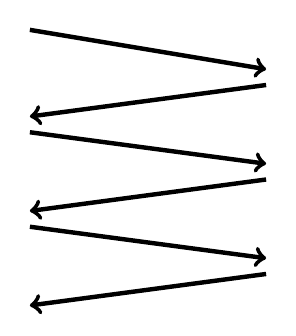
\begin{tikzpicture}

  % Message 1
  \node [coordinate] (a1) {};
  \node [coordinate,below right=0.5cm and 3cm of a1] (b1) {};
  \draw [->,ultra thick] (a1) -- node [above,midway] {} (b1);

  % Message 2
  \node [coordinate,below=0.2cm of b1] (b2) {};
  \node [coordinate,below left=0.4cm and 3cm of b2] (a2) {};
  \draw [->,ultra thick] (b2) -- node [above,midway] {} (a2);

  % Message 3
  \node [coordinate,below=0.2cm of a2] (a3) {};
  \node [coordinate,below right=0.4cm and 3cm of a3] (b3) {};
  \draw [->,ultra thick] (a3) -- node [above,midway] {} (b3);

  % Message 4
  \node [coordinate,below=0.2cm of b3] (b4) {};
  \node [coordinate,below left=0.4cm and 3cm of b4] (a4) {};
  \draw [->,ultra thick] (b4) -- node [above,midway] {} (a4);

  % Message 5
  \node [coordinate,below=0.2cm of a4] (a5) {};
  \node [coordinate,below right=0.4cm and 3cm of a5] (b5) {};
  \draw [->,ultra thick] (a5) -- node [above,midway] {} (b5);

  % Message 6
  \node [coordinate,below=0.2cm of b5] (b6) {};
  \node [coordinate,below left=0.4cm and 3cm of b6] (a6) {};
  \draw [->,ultra thick] (b6) -- node [above,midway] {} (a6);

\end{tikzpicture}
    \caption{}
  \end{subfigure}%
  \begin{subfigure}[t]{0.32\linewidth}
    \centering
    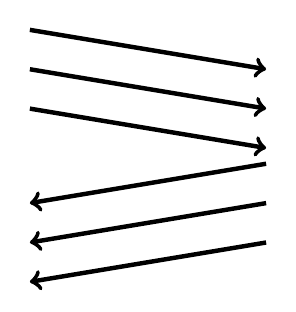
\begin{tikzpicture}

  % Message 1
  \node [coordinate] (a1) {};
  \node [coordinate,below right=0.5cm and 3cm of a1] (b1) {};
  \draw [->,ultra thick] (a1) -- node [above,midway] {} (b1);

  % Message 2
  \node [coordinate,below=0.5cm of a1] (a2) {};
  \node [coordinate,below right=0.5cm and 3cm of a2] (b2) {};
  \draw [->,ultra thick] (a2) -- node [above,midway] {} (b2);

  % Message 3
  \node [coordinate,below=0.5cm of a2] (a3) {};
  \node [coordinate,below right=0.5cm and 3cm of a3] (b3) {};
  \draw [->,ultra thick] (a3) -- node [above,midway] {} (b3);

  % Message 4
  \node [coordinate,below=0.2cm of b3] (b4) {};
  \node [coordinate,below left=0.5cm and 3cm of b4] (a4) {};
  \draw [->,ultra thick] (b4) -- node [above,midway] {} (a4);

  % Message 5
  \node [coordinate,below=0.5cm of b4] (b5) {};
  \node [coordinate,below left=0.5cm and 3cm of b5] (a5) {};
  \draw [->,ultra thick] (b5) -- node [above,midway] {} (a5);

  % Message 6
  \node [coordinate,below=0.5cm of b5] (b6) {};
  \node [coordinate,below left=0.5cm and 3cm of b6] (a6) {};
  \draw [->,ultra thick] (b6) -- node [above,midway] {} (a6);

\end{tikzpicture}
    \caption{}
  \end{subfigure}%
  \begin{subfigure}[t]{0.32\linewidth}
    \centering
    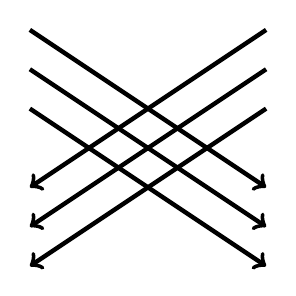
\begin{tikzpicture}

  % Message 1
  \node [coordinate] (a1) {};
  \node [coordinate,below right=2cm and 3cm of a1] (b1) {};
  \draw [->,ultra thick] (a1) -- node [above,midway] {} (b1);

  % Message 2
  \node [coordinate,below=0.5cm of a1] (a2) {};
  \node [coordinate,below right=2cm and 3cm of a2] (b2) {};
  \draw [->,ultra thick] (a2) -- node [above,midway] {} (b2);

  % Message 3
  \node [coordinate,below=0.5cm of a2] (a3) {};
  \node [coordinate,below right=2cm and 3cm of a3] (b3) {};
  \draw [->,ultra thick] (a3) -- node [above,midway] {} (b3);

  % Message 4
  \node [coordinate,right=3cm of a1] (b4) {};
  \node [coordinate,below left=2cm and 3cm of b4] (a4) {};
  \draw [->,ultra thick] (b4) -- node [above,midway] {} (a4);

  % Message 5
  \node [coordinate,below=0.5cm of b4] (b5) {};
  \node [coordinate,below left=2cm and 3cm of b5] (a5) {};
  \draw [->,ultra thick] (b5) -- node [above,midway] {} (a5);

  % Message 6
  \node [coordinate,below=0.5cm of b5] (b6) {};
  \node [coordinate,below left=2cm and 3cm of b6] (a6) {};
  \draw [->,ultra thick] (b6) -- node [above,midway] {} (a6);

\end{tikzpicture}
    \caption{}
  \end{subfigure}
  \caption[Message Traffic Pictographs]{Message Traffic Pictographs;
    Alternating Traffic (a), Unidirectional
    Traffic (b), Deferred Unidirectional Traffic (c)}
  \label{fig:picto}
\end{figure}

\section{Choice of Primitives}
\label{sec:choice-primitives}

In order to have fair conditions we use the same building blocks
in each protocol to build their respective primitives and
perform the benchmarks. The
codebase however is kept modular thus parts can be easily
exchanged if the need arises.
\begin{itemize}
\item \textbf{SHA-256.} As the hash functions and random
  oracles in each protocol. A possible alternative could be
  its successor SHA-3. SHA256 is part of the Go standard
  library \footnote{\url{https://golang.org/pkg/crypto/sha256/}}.
\item \textbf{AES-GCM~\cite{mcgrew2004security}.} As the authenticated
  encryption scheme with
  associated-data used among others in the FS-AEAD scheme in \cite{alwen2018double}.
  AES-GCM is also part of the Go standard
  library \footnote{\url{https://golang.org/pkg/crypto/aes/}}.
\item \textbf{Gentry-Silverberg HIBE~\cite{gentry2002hierarchical}.} As
  the HIBE scheme to build the ku-KEM in \cite{poettering2018towards} and
  the ku-PKE in \cite{jaeger2018optimal}. The use of HIBE schemes in
  cryptographic protocols is a relatively new idea thus there do not
  exist any industry-vetted implementations. The Gentry-Silverberg HIBE
  has thus been implemented by hand using a Go-port of the
  famous Stanford Pairing-Based Cryptography
  Library \footnote{\url{https://github.com/Nik-U/pbc}}.
  The Gentry-Silverberg construction is the most known scheme,
  the codebase also includes an experimental implementation of
  the Boneh-Boyen-Goh HIBE~\cite{boneh2005hierarchical} which however does
  not allow an unbounded
  depth as is required by both \cite{poettering2018towards} and
  \cite{jaeger2018optimal}.
\item \textbf{ECIES~\cite{shoup2001proposal}.} The Elliptic Curve Integrated
  Encryption Scheme on the standard curve P256 is used wherever a public-key
  encryption scheme is required. This is mainly due to the fact that
  some protocols have large and even growing messages sizes thus regular
  PKE schemes like RSA-OAEP or PKCS, where the message size is bounded
  depending on the modulus size, are not suited. ECIES is thus a
  relatively efficient alternative that can cope with messages
  of any size. This scheme has been implemented by hand.
\item \textbf{ECDSA~\cite{johnson2001elliptic}.} As the signature scheme in protocols where
  a regular or one-time signature is required. The primitive
  is mounted on the standard curve P256. ECDSA is part of the
  Go standard library \footnote{\url{https://golang.org/pkg/crypto/ecdsa/}}.
\item \textbf{Bellare et al.~Forward-Secure Signature~\cite{bellare1999forward}.}
  As part of the ku-Sig primitive in \cite{jaeger2018optimal}. It
  is the most known forward-secure signature scheme and has been implemented
  by hand.
\end{itemize}

To ease the labeling of the protocols within the plots we will
refer to them by using the first letters of their authors,
e.g.~Durak-Vaudenay is abbreviated to DV. Also note that
the plots contains two protocols more than discussed in
the previous section. DV-lite is the virtually equal to
the original protocol by Durak and Vaudenay it only replaces
the signcryption scheme with a symmetric-key variant in
this case an authenticated encryption scheme with associated
data, i.e.~AES-GCM in our case. Such a construction cannot provide
any post-compromise security but it significantly faster
than the regular protocol. The ACD-PK protocol goes the other way around
by adding a public-key encryption scheme and a digital signature
algorithm to the regular ACD protocol to plug some
of the post-compromise security holes caused by
the congruence of the states of both participants.
This comes at the cost of losing some efficiency.
These two additional protocols serve as baselines
to see how the metrics of a protocol can change when
some of its internals are replaced or extended. In the
following each benchmark is first given as plot then
analyzed below the figure.
The total number of
crypto-operations like encryptions and key updates
for $n$ operations is then also attached for each
primitive.

\section{Runtime Benchmarks}
\label{sec:runtime-benchmarks}

We start of by measuring the running time of the protocols. As
it is practice when it comes to pinpointing time in software
benchmarks the Go profiler runs the benchmarks repeatedly
until the average time over all runs stabilizes. Usually
earlier runs serve as warm-ups to bring all the program
data into the cache for faster access in later runs.
Due to the large differences in terms
of runtimes between the protocols the y-axis is
in logarithmic scale.
Note that in the below listings invocations of
hash functions have been omitted.
Also note that the measurements were only conducted up
to 900 messages anything beyond can then be safely extrapolated.

\subsection{Alternating Traffic}
\label{sec:alternating-traffic}

\begin{figure}[H]
  \centering
  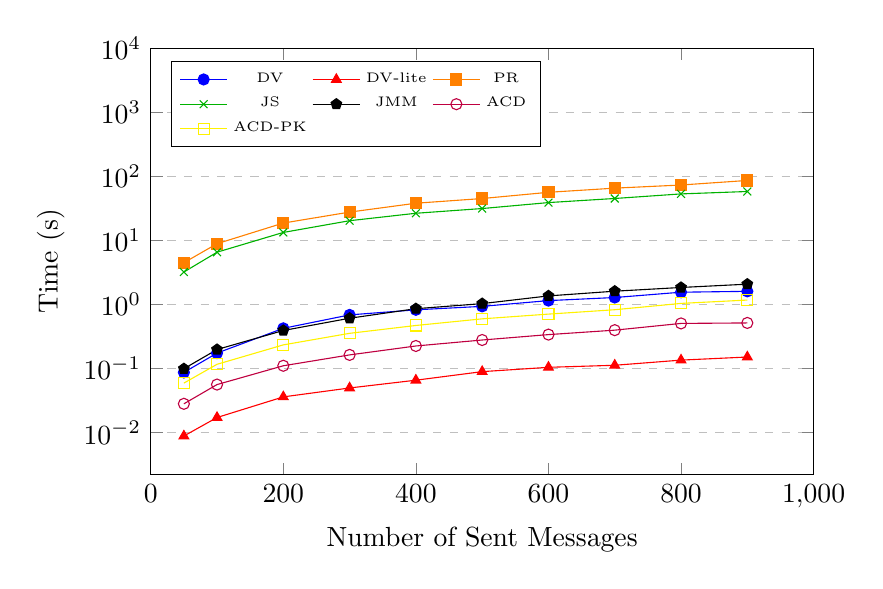
\begin{tikzpicture}[scale=1]
\begin{axis}[
  %title=Alternating,
  ymode=log,
  legend style={font=\tiny, legend columns=3},
  scaled ticks=false,
  xlabel={Number of Sent Messages},
  ylabel={Time (s)},
  xmin=0, xmax=1000,
  ymax=10000,
  xtick={0,200,400,600,800,1000},
  ytick={0.01,0.1,1,10,100,1000,10000},
  legend pos=north west,
  ymajorgrids=true,
  xminorticks=false,
  yminorticks=false,
  grid style=dashed,
  height=7cm,
  width=10cm,
]
 
\addplot[color=blue,mark=*]
   coordinates {
  (50,0.0874)(100,0.175)(200,0.426)(300,0.690)(400,0.828)(500,0.938)(600,1.153)
  (700,1.288)(800,1.559)(900,1.609)
  };

\addplot[color=red,mark=triangle*]
  coordinates {
  (50,0.0089)(100,0.0173)(200,0.0363)(300,0.0500)(400,0.0661)(500,0.0899)
  (600,0.105)(700,0.113)(800,0.136)(900,0.152)
  };

\addplot[color=orange,mark=square*]
  coordinates {
  (50,4.5)(100,8.9)(200,18.7)(300,27.7)(400,38.1)(500,45.1)
  (600,56.4)(700,65.5)(800,73.3)(900,86.3)
  };

\addplot[color=black!30!green,mark=x]
  coordinates {
  (50,3.217)(100,6.560)(200,13.343)(300,20.338)(400,26.564)(500,31.485)
  (600,38.999)(700,45.183)(800,53.249)(900,58.065)
  };

\addplot[color=black,mark=pentagon*]
  coordinates {
  (50,0.0998)(100,0.199)(200,0.394)(300,0.612)(400,0.862)(500,1.035)
  (600,1.365)(700,1.617)(800,1.848)(900,2.081)
  };

\addplot[color=purple,mark=o]
  coordinates {
  (50,0.0283)(100,0.0565)(200,0.111)(300,0.164)(400,0.226)(500,0.280)
  (600,0.340)(700,0.399)(800,0.508)(900,0.517)
  };

\addplot[color=yellow,mark=square]
  coordinates {
  (50,0.0596)(100,0.117)(200,0.235)(300,0.356)(400,0.472)(500,0.599)
  (600,0.710)(700,0.831)(800,1.043)(900,1.176)
  };

  \legend{DV,DV-lite,PR,JS,JMM,ACD,ACD-PK}
 
\end{axis}
\end{tikzpicture} 
  \caption{Runtime Benchmark Alternating Traffic}
  \label{fig:time-alt}
\end{figure}

\begin{itemize}
\item \textbf{PR.} Since the unidirectional period is exactly one,
  the epoch counters $(E_S,E_R)$ for both user also have difference one
  thus each user will perform exactly two encryptions, except for the
  first exchange, for each message.
  Furthermore, there are no key updates in the receive function because
  the users will only use the keys they exchanged to encrypt and decrypt
  functions.
  \begin{center}
    \begin{tabular}{ | l | l | l | l |}
    \hline
    Primitive & Generations & (Encs/Decs) $\vee$ (Sigs/Vers) & Updates PK/SK \\ \hline
    \textbf{ku-KEM} & $2n$ & $2n-1/2n-1$ & $0/0$ \\ \hline
    \textbf{Signature} & $n$ & $n/n$ & - \\  
    \hline
    \end{tabular}
  \end{center}
\item \textbf{JS.} We have a similar situation with the Jaeger and Stepanovs
  protocol. Both participants take turns updating their ku-PKE and
  ku-Sig keys once while exchanging new key pairs. Since the direction
  of traffic is changing after one message the encryption key $ek'$
  is never updated. All of this results in a similar running time
  than the previous protocol.
  \begin{center}
    \begin{tabular}{ | l | l | l | l |}
    \hline
    Primitive & Generations & (Encs/Decs) $\vee$ (Sigs/Vers) & Updates PK/SK \\ \hline
    \textbf{ku-PKE} & $0$ & $n/n$ & $0/n$ \\ \hline
    \textbf{ku-Sig} & $0$ & $n/n$ & $n-1/n$ \\  
    \hline
    \end{tabular}
  \end{center}
\item \textbf{DV.} Each participant will perform two onion encryptions
  for each message which translates to two signcryption
  encryptions/decryptions. Since the signcryption scheme is spun up by combining
  a regular PKE system and a DSS scheme we have two PKE encryptions/decryptions
  and two DSS signatures/verifications per message, excluding
  the first message by Alice. Also note that
  only one key generation is performed during the onion encryption.
  Replacing the signcryption algorithm with a symmetric AEAD scheme
  will result in a protocol that has a runtime well below one second
  even for 900 messages.
  \begin{center}
    \begin{tabular}{ | l | l | l | l |}
    \hline
    Primitive & Generations & (Encs/Decs) $\vee$ (Sigs/Vers) & Updates PK/SK \\ \hline
    \textbf{PKE} & $2n$ & $2n-1/2n-1$ & $0/0$ \\ \hline
    \textbf{Signature} & $2n-1$ & $2n-1/2n-1$ & $0/0$ \\  
    \hline
    \end{tabular}
  \end{center}
\item \textbf{JMM.} Superficially we have single calls to the hku-PKE, ku-Sig and
  Sig primitives but the magic happens under the hood within the hku-PKE and can
  be checked in the original paper (see page 23). We have the following distribution
  of operations throughout the primitives. To keep the notation lightweight
  the generation of update information \texttt{UpdGen} as part
  of the hku-PKE scheme is counted as a key generation call.
  \begin{center}
    \begin{tabular}{ | l | l | l | l |}
    \hline
    Primitive & Generations & (Encs/Decs) $\vee$ (Sigs/Vers) & Updates PK/SK \\ \hline
    \textbf{ku-Sig} & $0$ & $n/n$ & - \\ \hline
    \textbf{sku-PKE} & $2n$ & $n/n$ & $n/n$ \\ \hline
    \textbf{PKE-AD} & $3n$ & $n/n$ & - \\
    \hline
    \end{tabular}
  \end{center}
\item \textbf{ACD.} The protocol only contains loops for housekeeping operations
  like the deletion of states but not for cryptographic operations. It performs
  better than the previous two protocols due to only using public-key cryptography
  for the continuous key agreement primitive. The CKA operations are counted
  as key generation calls. Also since the participants are alternating,
  each message marks the start of a new epoch thus the key agreement and
  FS-AEAD key generations are executed with each call. The addition
  of public-key schemes in ACD-PK adds two generation calls, an PKE encryption call,
  and DSS signature call to the send function and their corresponding
  decryption/verification calls to the receive function hence more
  resembling the DV and JMM protocols in terms of runtime.
  \begin{center}
    \begin{tabular}{ | l | l | l | l |}
    \hline
    Primitive & Generations & (Encs/Decs) $\vee$ (Sigs/Vers) & Updates PK/SK \\ \hline
    \textbf{FS-AEAD} & $2n$ & $n/n$ & - \\ \hline
    \textbf{CKA} & $2n$ & - & - \\  
    \hline
    \end{tabular}
  \end{center}
\end{itemize}

We have a tame and contained behaviour when the participants
alternate their messages. This results in three relatively fast
protocols (DV, JMM, ACD) and two moderately slow protocols
(PR, JS) that rely on HIBE schemes, which was to be
expected.

\clearpage

\subsection{Unidirectional Traffic}
\label{sec:unid-traff}

\begin{figure}[H]
  \centering
  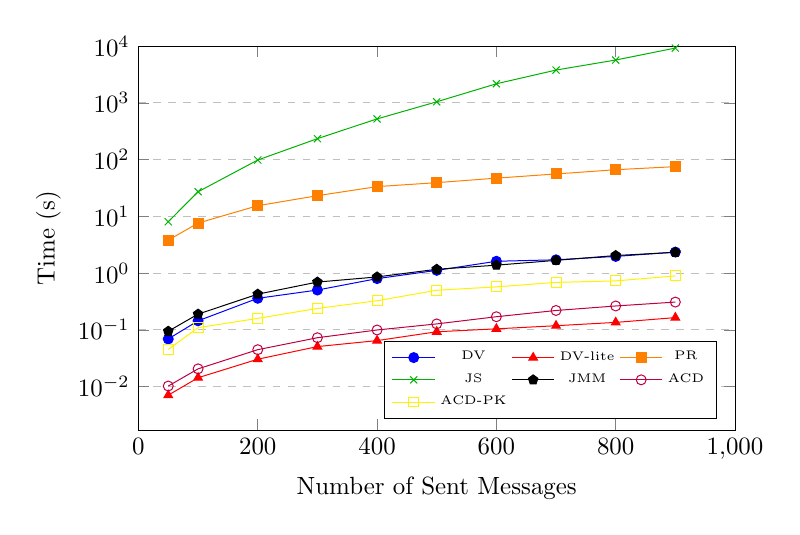
\begin{tikzpicture}[scale=0.9]
\begin{axis}[
  ymode=log,
 legend style={font=\tiny, legend columns=3},
  scaled ticks=false,
  xlabel={Number of Sent Messages},
  ylabel={Time (s)},
  xmin=0, xmax=1000,
  ymax=10000,
  xtick={0,200,400,600,800,1000},
  ytick={0.01,0.1,1,10,100,1000,10000},
  legend pos=south east,
  ymajorgrids=true,
  xminorticks=false,
  yminorticks=false,
  grid style=dashed,
  height=7cm,
  width=10cm,
]
 
\addplot[color=blue,mark=*]
   coordinates {
  (50,0.0689)(100,0.144)(200,0.359)(300,0.502)(400,0.798)(500,1.116)(600,1.614)
  (700,1.712)(800,1.965)(900,2.344)
  };

\addplot[color=red,mark=triangle*]
  coordinates {
  (50,0.00704)(100,0.0143)(200,0.0303)(300,0.0506)(400,0.0645)(500,0.0923)
  (600,0.104)(700,0.118)(800,0.135)(900,0.164)
  };

\addplot[color=orange,mark=square*]
  coordinates {
  (50,3.8)(100,7.6)(200,15.4)(300,23.1)(400,33.4)(500,39.2)
  (600,47.1)(700,55.8)(800,66.3)(900,75.1)
  };

\addplot[color=black!30!green,mark=x]
  coordinates {
  (50,8.024)(100,27.096)(200,98.210)(300,233.751)(400,521.110)(500,1044.091)
  (600,2168.099)(700,3783.724)(800,5688.493)(900,9235.921)
  };

\addplot[color=black,mark=pentagon*]
  coordinates {
  (50,0.0943)(100,0.189)(200,0.425)(300,0.694)(400,0.854)(500,1.166)
  (600,1.377)(700,1.675)(800,2.036)(900,2.319)
  };

\addplot[color=purple,mark=o]
  coordinates {
  (50,0.0102)(100,0.0205)(200,0.0446)(300,0.0725)(400,0.0992)(500,0.127)
  (600,0.170)(700,0.219)(800,0.263)(900,0.308)
  };

\addplot[color=yellow,mark=square]
  coordinates {
  (50,0.0451)(100,0.109)(200,0.159)(300,0.238)(400,0.325)(500,0.498)
  (600,0.571)(700,0.685)(800,0.727)(900,0.891)
  };

  \legend{DV,DV-lite,PR,JS,JMM,ACD,ACD-PK}
 
\end{axis}
\end{tikzpicture} 
  \caption{Runtime Benchmark Unidirectional Traffic}
  \label{fig:time-uni}
\end{figure}

\begin{itemize}
\item \textbf{PR.} The unidirectional case is similar to the alternating
  one. Again there are no key updates. Alice who sends the first
  $\frac{n}{2}$ tranches will only do a single encryption for
  each message but both participants will accumulate the keys
  generated and distributed by Alice. This means the first
  message the Bob sends will use all those keys for the encryption
  and Alice will use all keys for the decryption. Every following
  message by Bob will then be only encrypted once. All of this
  makes the unidirectional traffic slightly faster than the alternating.
  \begin{center}
    \begin{tabular}{ | l | l | l | l |}
    \hline
    Primitive & Generations & (Encs/Decs) $\vee$ (Sigs/Vers) & Updates PK/SK \\ \hline
    \textbf{ku-KEM} & $2n$ & $\frac{3}{2}n/\frac{3}{2}n$ & $0/0$ \\ \hline
    \textbf{Signature} & $n$ & $n/n$ & - \\  
    \hline
    \end{tabular}
  \end{center}
\item  \textbf{JS.} Contrary to all others the protocol by Jaeger and Stepanovs incurs a
  quadratic ku-PKE key-update penalty for repeated sending without receiving.
  Each send operation will perform one \texttt{ku-PKE.UpdEk} call more than the previous
  one since the partner will update the corresponding decryption key
  in any case. This gives $\frac{(n-1)n}{2}$ \texttt{ku-PKE.UpdEk} and
  $\frac{n}{2}$ \texttt{ku-PKE.UpdDk} updates per user. Furthermore,
  since Bob updates his ku-Sig signature key in every receive, Alice
  has to perform $n$ \texttt{ku-Sig.UpdVk} calls when she receives the
  first message from Bob. The protocol thus performs significantly worse in unidirectional
  traffic than alternating.
  \begin{center}
    \begin{tabular}{ | l | l | l | l |}
    \hline
    Primitive & Generations & (Encs/Decs) $\vee$ (Sigs/Vers) & Updates PK/SK \\ \hline
    \textbf{ku-PKE} & $0$ & $n/n$ & $\frac{(n-1)n}{2}/n$ \\ \hline
    \textbf{ku-Sig} & $0$ & $n/n$ & $\frac{n}{2}/n$ \\  
    \hline
    \end{tabular}
  \end{center}
\item \textbf{DV.} All messages by Alice have a single onion layer except
  the first message travelling in the opposite direction for which both
  participants use $\frac{n}{2}$ onion
  layers using all accumulated signcryption keys. The resulting runtime
  is thus slightly better than in the alternating case.
  \begin{center}
    \begin{tabular}{ | l | l | l | l |}
    \hline
    Primitive & Generations & (Encs/Decs) $\vee$ (Sigs/Vers) & Updates PK/SK \\ \hline
    \textbf{PKE} & $2n$ & $\frac{3}{2}n/\frac{3}{2}n$ & $0/0$ \\ \hline
    \textbf{Signature} & $2n$ & $\frac{3}{2}n/\frac{3}{2}n$ & $0/0$ \\  
    \hline
    \end{tabular}
  \end{center}
\item \textbf{JMM.} Unidirectional traffic does not change the metrics
  with respect to alternating traffic for this protocol thus we have the
  same amount of operations for both. This is due to the fact that in
  the hku-PKE the sku-PKE key pairs are only updated once per transmission
  if there are no messages in delay as it is the case with alternating
  and unidirectional traffic.
  \begin{center}
    \begin{tabular}{ | l | l | l | l |}
    \hline
    Primitive & Generations & (Encs/Decs) $\vee$ (Sigs/Vers) & Updates PK/SK \\ \hline
    \textbf{ku-Sig} & $0$ & $n/n$ & - \\ \hline
    \textbf{sku-PKE} & $2n$ & $n/n$ & $n/n$ \\ \hline
    \textbf{PKE-AD} & $3n$ & $n/n$ & - \\
    \hline
    \end{tabular}
  \end{center}
\item \textbf{ACD.} Alice starts a new epoch with her first message, the
  same for Bob with his first message after receiving the $\frac{n}{2}$
  from Alice. This results in a total of $4$ CKA calls and $4$ FS-AEAD
  key generations making it even faster than it already was in alternating
  traffic.
  \begin{center}
    \begin{tabular}{ | l | l | l | l |}
    \hline
    Primitive & Generations & (Encs/Decs) $\vee$ (Sigs/Vers) & Updates PK/SK \\ \hline
    \textbf{FS-AEAD} & $4$ & $n/n$ & - \\ \hline
    \textbf{CKA} & $4$ & - & - \\  
    \hline
    \end{tabular}
  \end{center}
\end{itemize}

We can see that in unidirectional traffic there is a clear separation
between protocols of Poettering/Rösler and Jaeger/Stepanovs due
to the quadratic penalty of encryption key updates within the
key-updatable PKE. All the other protocols have more or less
the same metrics as in alternating traffic.

\clearpage

\subsection{Deferred Unidirectional Traffic}
\label{sec:deferr-unid-traff-1}

\begin{figure}[H]
  \centering
  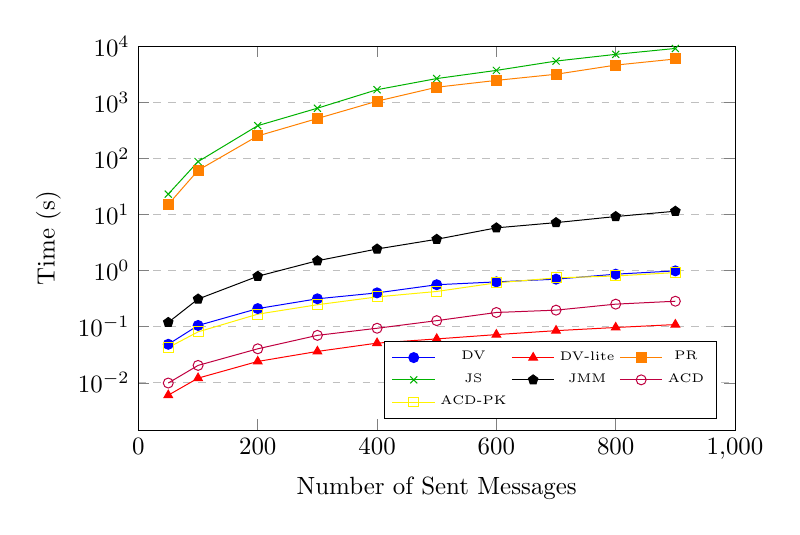
\begin{tikzpicture}[scale=0.9]
\begin{axis}[
  ymode=log,
  legend style={font=\tiny, legend columns=3},
  scaled ticks=false,
  xlabel={Number of Sent Messages},
  ylabel={Time (s)},
  xmin=0, xmax=1000,
  ymax=10000,
  xtick={0,200,400,600,800,1000},
  ytick={0.01,0.1,1,10,100,1000,10000},
  legend pos=south east,
  ymajorgrids=true,
  xminorticks=false,
  yminorticks=false,
  grid style=dashed,
  height=7cm,
  width=10cm,
]
 
\addplot[color=blue,mark=*]
   coordinates {
  (50,0.0485)(100,0.105)(200,0.210)(300,0.314)(400,0.400)(500,0.559)(600,0.628)
  (700,0.702)(800,0.862)(900,0.987)
  };

\addplot[color=red,mark=triangle*]
  coordinates {
  (50,0.00601)(100,0.0121)(200,0.0240)(300,0.0362)(400,0.0509)(500,0.0605)
  (600,0.0722)(700,0.0849)(800,0.0967)(900,0.109)
  };

\addplot[color=orange,mark=square*]
  coordinates {
  (50,15.052)(100,61.132)(200,250.773)(300,512.437)(400,1043.941)(500,1849.874)
  (600,2449.326)(700,3149.923)(800,4587.110)(900,5897.349)
  };


\addplot[color=black!30!green,mark=x]
  coordinates {
  (50,23.084)(100,87.370)(200,382.419)(300,782.271)(400,1672.800)(500,2640.221)
  (600,3691.952)(700,5413.382)(800,7129.012)(900,9087.283)
  };

\addplot[color=black,mark=pentagon*]
  coordinates {
  (50,0.119)(100,0.311)(200,0.791)(300,1.496)(400,2.421)(500,3.608)
  (600,5.770)(700,7.148)(800,9.172)(900,11.411)
  };

\addplot[color=purple,mark=o]
  coordinates {
  (50,0.0099)(100,0.0204)(200,0.0403)(300,0.0700)(400,0.0937)(500,0.128)
  (600,0.179)(700,0.197)(800,0.252)(900,0.284)
  };

\addplot[color=yellow,mark=square]
  coordinates {
  (50,0.0424)(100,0.0808)(200,0.167)(300,0.246)(400,0.339)(500,0.424)
  (600,0.604)(700,0.740)(800,0.801)(900,0.920)
  };

    
  \legend{DV,DV-lite,PR,JS,JMM,ACD,ACD-PK}
 
\end{axis}
\end{tikzpicture} 
  \caption{Runtime Benchmark Deferred Unidirectional Traffic}
  \label{fig:time-def-uni}
\end{figure}

\begin{itemize}
\item \textbf{PR.} As in the regular unidirectional traffic both
  participants will encrypt each message only once. However, for
  each received message a participant will update all
  the $\frac{n}{2}$ accumulated keys resulting in $2(\frac{n}{2})^2$
  HIBE extractions and a update key update complexity of $\mathcal{O}(n^2)$.
  Deferred unidirectional traffic is thus significantly slower than
  regular unidirectional.
  \begin{center}
    \begin{tabular}{ | l | l | l | l |}
    \hline
    Primitive & Generations & (Encs/Decs) $\vee$ (Sigs/Vers) & Updates PK/SK \\ \hline
    \textbf{ku-KEM} & $2n$ & $n/n$ & $2(\frac{n}{2})^2/2(\frac{n}{2})^2$ \\ \hline
    \textbf{Signature} & $n$ & $n/n$ & - \\  
    \hline
    \end{tabular}
  \end{center}
\item \textbf{JS.} Deferred unidirectional traffic incurs a quadratic
  penalty for both ku-PKE key updates. A participant
  will update all the accumulated ku-PKE decryption keys for
  each received message, in total $n(\frac{n}{2}+1)$ calls.
  Updating the encryption key has the same complexity as in the
  regular unidirectional case. This means that the protocol
  performs the worst in deferred unidirectional traffic.
  \begin{center}
    \begin{tabular}{ | l | l | l | l |}
    \hline
    Primitive & Generations & (Encs/Decs) $\vee$ (Sigs/Vers) & Updates PK/SK \\ \hline
    \textbf{ku-PKE} & $0$ & $n/n$ & $\frac{(n-1)n}{2}/n(\frac{n}{2}+1)$ \\ \hline
    \textbf{ku-Sig} & $0$ & $n/n$ & $0/n$ \\  
    \hline
    \end{tabular}
  \end{center}
\item \textbf{DV.} In deferred unidirectional traffic it is easy to see that
  all messages have a single onion layer thus resulting $n$ overall
  signcryption calls. Note however that the first message
  by either participant after receiving all message will perform
  $\frac{n}{2}$ onion encryptions. This is not captured
  by this benchmark.
  \begin{center}
    \begin{tabular}{ | l | l | l | l |}
    \hline
    Primitive & Generations & (Encs/Decs) $\vee$ (Sigs/Vers) & Updates PK/SK \\ \hline
    \textbf{PKE} & $2n$ & $n/n$ & $0/0$ \\ \hline
    \textbf{Signature} & $2n$ & $n/n$ & $0/0$ \\  
    \hline
    \end{tabular}
  \end{center}
\item \textbf{JMM.} In deferred unidirectional traffic the protocol
  has a quadratic sku-PKE key update penalty in \texttt{hku-PKE.Dec} and
  \texttt{hku-PKE.BcUpdEk}. For each received message
  both participants update all the accumulated keys, hence it performs
  significantly worse than the protocol by Durak and Vaudenay.
  \begin{center}
    \begin{tabular}{ | l | l | l | l |}
    \hline
    Primitive & Generations & (Encs/Decs) $\vee$ (Sigs/Vers) & Updates PK/SK \\ \hline
    \textbf{ku-Sig} & $0$ & $n/n$ & - \\ \hline
    \textbf{sku-PKE} & $2n$ & $n/n$ & $n+2n^2/n+2n^2$ \\ \hline
    \textbf{PKE-AD} & $3n$ & $n/n$ & - \\
    \hline
    \end{tabular}
  \end{center}
\item \textbf{ACD.} We have a similar situation with respect to regular
  unidirectional traffic. The only difference is that Bob does not
  start a new epoch with his first message, hence we save two CKA calls
  and two FS-AEAD key generations.
  \begin{center}
    \begin{tabular}{ | l | l | l | l |}
    \hline
    Primitive & Generations & (Encs/Decs) $\vee$ (Sigs/Vers) & Updates PK/SK \\ \hline
    \textbf{FS-AEAD} & $2$ & $n/n$ & - \\ \hline
    \textbf{CKA} & $2$ & - & - \\  
    \hline
    \end{tabular}
  \end{center}
\end{itemize}

In deferred unidirectional traffic it now also possible to separate
the protocols Durak/Vaudenay and Jost/Maurer/Mularczyk due to
the quadratic key update complexity within the
hku-PKE scheme. The protocol by Poettering
and Rösler also sees a jump in complexity caused by another
quadratic update complexity. In summary, it is now obvious that
the protocols by Poettering/Rösler and Jaeger/Stepanovs are prohibitively
inefficient especially in unidirectional traffic. Furthermore,
as expected the Double Ratchet outperforms the other protocols,
although offering weaker security guarantees. It then boils down
to a case-by-base decision on how to choose the
proper trade off between security and performance.

\section{Message Size Benchmarks}
\label{sec:ciph-size-benchm}

The size of the message is another viable metric in order to
judge a messaging or key-agreement protocol. Smaller messages save disk space,
are easier to transmit over the network and take generally
less time to process. We again consider the traffic
types from the previous section and measure the maximal
size in bytes that any message reaches. The size
naturally depends on how much data is packed into the message
but also on the primitives used to generate this data.
For the messaging protocols the plaintext and associated
data size is fixed at \textbf{64 bytes}.

\clearpage

\subsection{Alternating Traffic}
\label{sec:alternating-traffic-1}

\begin{figure}[H]
  \centering
  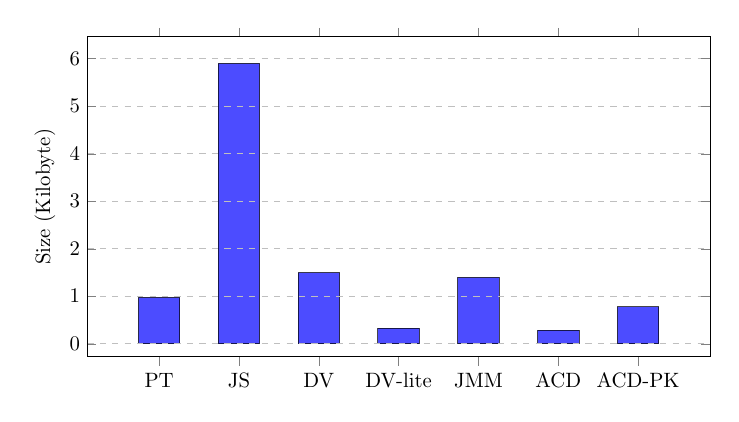
\begin{tikzpicture}[scale=.75]
  \begin{axis} [
    ybar, axis on top,
    bar width= 20pt,
    legend pos=north west,
    ylabel={Size (Kilobyte)},
    symbolic x coords={PT,JS,DV, DV-lite, JMM, ACD, ACD-PK},
    xtick=data,
    ytick={0,1,2,3,4,5,6},
    nodes near coords={},
    grid style=dashed,
    ymajorgrids=true,
    yminorticks=false,
    xminorticks=false,
    legend style={at={(0.5,1)},
    anchor=north,legend columns=-1},
    %xticklabel style = {rotate=75},
    height=7cm,
    width=\textwidth,
    enlarge x limits=0.15,
  ]

   y=-0.5cm,      \addplot [
      fill=blue,
      opacity=0.7,
      area legend,
    ] coordinates {
        (PT,0.98)
        (JS,5.9)
        (DV,1.5)
	(DV-lite,0.33)
        (JMM,1.4)
        (ACD,0.29)
        (ACD-PK,0.78)
    };

%    \addplot [
%      fill=purple,
%      opacity=0.7,
%      area legend,
%    ] coordinates {
%        (Alternating,3260.4) +- (0,47.432291)
%        (Unidirectional,6148.4) +- (0,112.415104)
%        (Def. Unidirectional,10852.9) +- (0,43.195807)
%    };
%    
%    \addplot [
%      fill=red,
%      opacity=0.7,
%      area legend,
%    ] coordinates {
%        (Alternating,33459.41112) +- (0,592.258861)
%        (Unidirectional,64690.703011) +- (0,1429.674333)
%        (Def. Unidirectional,131962.165976) +- (0,911.453089)
%    };
%
%   \addplot [
%      fill=red,
%      opacity=0.7,
%      area legend,
%    ] coordinates {
%        (Alternating,33459.41112) +- (0,592.258861)
%        (Unidirectional,64690.703011) +- (0,1429.674333)
%        (Def. Unidirectional,131962.165976) +- (0,911.453089)
%    };
%
%       \addplot [
%      fill=orange,
%      opacity=0.7,
%      area legend,
%    ] coordinates {
%        (Alternating,33459.41112) +- (0,592.258861)
%        (Unidirectional,64690.703011) +- (0,1429.674333)
%        (Def. Unidirectional,131962.165976) +- (0,911.453089)
%    };
%
%       \addplot [
%      fill=yellow,
%      opacity=0.7,
%      area legend,
%    ] coordinates {
%        (Alternating,33459.41112) +- (0,592.258861)
%        (Unidirectional,64690.703011) +- (0,1429.674333)
%        (Def. Unidirectional,131962.165976) +- (0,911.453089)
%    };
%
%     \addplot [
%      fill=green,
%      opacity=0.7,
%      area legend,
%    ] coordinates {
%        (Alternating,33459.41112) +- (0,592.258861)
%        (Unidirectional,64690.703011) +- (0,1429.674333)
%        (Def. Unidirectional,131962.165976) +- (0,911.453089)
%    };

%    \legend{PR, JS, DV, DV-lite, JMM, ACD, ACD-PK}
  \end{axis}
\end{tikzpicture} 
  \caption{Message Size Benchmark Alternating Traffic}
  \label{fig:msg-size}
\end{figure}

In alternating traffic the states are continuously flushed causing the
message size to be constant for all number of number
of exchanged messages. The large number of the JS protocol
is primarily caused by the forward-secure signature scheme
whose keys and signatures are larger than in a regular signature scheme.
Also note that in the DV protocol two onion encryptions
are performed for each message causing a swollen
ciphertext. Naturally, the two protocols using
symmetric primitives compete for the lowest message size.

\subsection{Unidirectional Traffic}
\label{sec:unid-traff-1}

\begin{figure}[H]
  \centering
  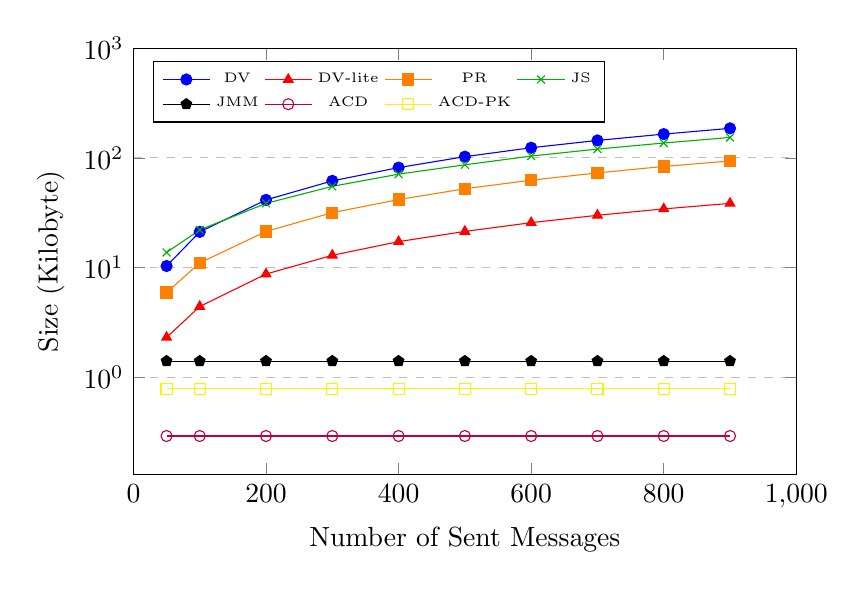
\begin{tikzpicture}[scale=1]
\begin{axis}[
  %ymode=log,
%  legend style={font=\tiny, legend columns=4},
%  scaled ticks=false,
%  xlabel={Number of Sent Messages},
%  ylabel={Size (Kilobyte)},
%  xmin=0, xmax=1000,
%  ymax=200,
%  xtick={0,200,400,600,800,1000},
%  %ytick={0.01,0.1,1,10,100,1000,10000},
%  ytick={0,20,40,60,80,100,120,140,160,180,200},
%  legend pos=north west,
%  ymajorgrids=true,
%  xminorticks=false,
%  yminorticks=false,
%  grid style=dashed,
%  height=7cm,
%  width=10cm,
  ymode=log,
  legend style={font=\tiny, legend columns=4},
  scaled ticks=false,
  xlabel={Number of Sent Messages},
  ylabel={Size (Kilobyte)},
  xmin=0, xmax=1000,
  ymax=1000,
  xtick={0,200,400,600,800,1000},
  ytick={0.001,0.01,0.1,1,10,100,1000},
  %ytick={0,20,40,60,80,100,120,140,160,180,200},
  legend pos=north west,
  ymajorgrids=true,
  xminorticks=false,
  yminorticks=false,
  grid style=dashed,
  height=7cm,
  width=10cm,
]
 
\addplot[color=blue,mark=*]
   coordinates {
  (50,10.3)(100,21.1)(200,41.3)(300,61.6)(400,81.4)(500,102.4)(600,123.5)
  (700,144.0)(800,164.5)(900,185.6)
  };

\addplot[color=red,mark=triangle*]
  coordinates {
  (50,2.3)(100,4.4)(200,8.7)(300,12.9)(400,17.2)(500,21.3)
  (600,25.6)(700,29.9)(800,34.2)(900,38.4)
  };

\addplot[color=orange,mark=square*]
  coordinates {
  (50,5.9)(100,11.0)(200,21.3)(300,31.6)(400,41.6)(500,52.2)
  (600,62.5)(700,72.8)(800,83.4)(900,93.5)
  };


\addplot[color=black!30!green,mark=x]
  coordinates {
  (50,13.7)(100,22.0)(200,38.4)(300,54.9)(400,70.9)(500,86.3)
  (600,103.7)(700,120.1)(800,136.4)(900,153.3)
  };

\addplot[color=black,mark=pentagon*]
  coordinates {
  (50,1.4)(100,1.4)(200,1.4)(300,1.4)(400,1.4)(500,1.4)
  (600,1.4)(700,1.4)(800,1.4)(900,1.4)
  };

\addplot[color=purple,mark=o]
  coordinates {
  (50,0.29)(100,0.29)(200,0.29)(300,0.29)(400,0.29)(500,0.29)
  (600,0.29)(700,0.29)(800,0.29)(900,0.29)
  };

\addplot[color=yellow,mark=square]
  coordinates {
  (50,0.78)(100,0.78)(200,0.78)(300,0.78)(400,0.78)(500,0.78)
  (600,0.78)(700,0.78)(800,0.78)(900,0.78)
  };


  \legend{DV,DV-lite,PR,JS,JMM,ACD,ACD-PK}
 
\end{axis}
\end{tikzpicture} 
  \caption{Message Size Benchmark Unidirectional Traffic}
  \label{fig:msg-size-uni}
\end{figure}

Note that we have a constant ciphertext size for the JMM and ACD
protocols.
The effects of the onion encryption are now clearly visible
in the DV protocol. Recall that in unidirectional traffic
the first message in the opposite direction requires $\frac{n}{2}$
onion encryptions incurring a large ciphertext size for
this particular message.
There similar situation takes place in the PR protocol where
the first message in the opposite direction
will have $\frac{n}{2}$ ciphertexts attached to the message.
Finally, the quadratic key updates in the JS protocol
have a deep HIBE hierarchy as a consequence that
enlarges the ciphertexts as well as the HIBE
keys.

\subsection{Deferred Unidirectional Traffic}
\label{sec:deferr-unid-traff}

\begin{figure}[H]
  \centering
  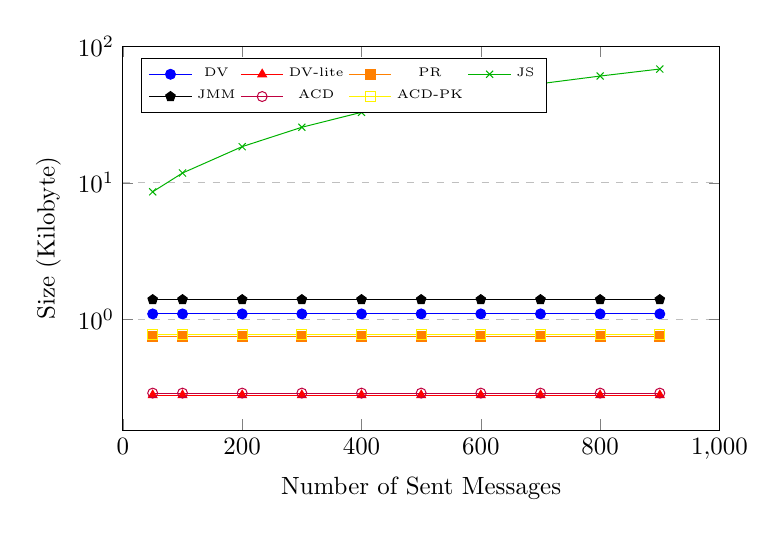
\begin{tikzpicture}[scale=0.9]
\begin{axis}[
  ymode=log,
  legend style={font=\tiny, legend columns=4},
  scaled ticks=false,
  xlabel={Number of Sent Messages},
  ylabel={Size (Kilobyte)},
  xmin=0, xmax=1000,
  ymax=100,
  xtick={0,200,400,600,800,1000},
  ytick={0.001,0.01,0.1,1,10,100},
  %ytick={0,20,40,60,80,100,120,140,160,180,200},
  legend pos=north west,
  ymajorgrids=true,
  xminorticks=false,
  yminorticks=false,
  grid style=dashed,
  height=7cm,
  width=10cm,
]
 
\addplot[color=blue,mark=*]
   coordinates {
  (50,1.1)(100,1.1)(200,1.1)(300,1.1)(400,1.1)(500,1.1)(600,1.1)
  (700,1.1)(800,1.1)(900,1.1)
  };

\addplot[color=red,mark=triangle*]
  coordinates {
  (50,0.28)(100,0.28)(200,0.28)(300,0.28)(400,0.28)(500,0.28)
  (600,0.28)(700,0.28)(800,0.28)(900,0.28)
  };

\addplot[color=orange,mark=square*]
  coordinates {
  (50,0.75)(100,0.75)(200,0.75)(300,0.75)(400,0.75)(500,0.75)
  (600,0.75)(700,0.75)(800,0.75)(900,0.75)
  };

\addplot[color=black!30!green,mark=x]
  coordinates {
  (50,8.6)(100,11.8)(200,18.4)(300,25.5)(400,32.8)(500,39.9)
  (600,46.3)(700,53.1)(800,60.4)(900,68.0)
  };

\addplot[color=black,mark=pentagon*]
  coordinates {
  (50,1.4)(100,1.4)(200,1.4)(300,1.4)(400,1.4)(500,1.4)
  (600,1.4)(700,1.4)(800,1.4)(900,1.4)
  };

\addplot[color=purple,mark=o]
  coordinates {
  (50,0.29)(100,0.29)(200,0.29)(300,0.29)(400,0.29)(500,0.29)
  (600,0.29)(700,0.29)(800,0.29)(900,0.29)
  };

\addplot[color=yellow,mark=square]
  coordinates {
  (50,0.78)(100,0.78)(200,0.78)(300,0.78)(400,0.78)(500,0.78)
  (600,0.78)(700,0.78)(800,0.78)(900,0.78)
  };

  \legend{DV,DV-lite,PR,JS,JMM,ACD,ACD-PK}
 
\end{axis}
\end{tikzpicture} 
  \caption{Message Size Benchmark Deferred Unidirectional Traffic}
  \label{fig:msg-size-def}
\end{figure}

In deferred unidirectional traffic the DV and PR now also
have a constant message size so the protocol by
Jaeger and Stepanovs is the only one with a linearly
growing message size due to the repeated key updates
during unidirectional traffic.

\section{State Size Benchmarks}
\label{sec:state-size-benchm}

The last metric we investigate is the size of a user state during
alternating, unidirectional and deferred unidirectional
traffic. Preferably, a state should only occupy small amounts of
memory making the surrounding protocol suitable for small devices with
limited amounts of memory otherwise data needs to be swapped from and
to the disk degrading the overall performance. Again we only
measure the maximal size in bytes a state reaches during the benchmark.

\subsection{Alternating Traffic}
\label{sec:alternating-traffic-2}

\begin{figure}[H]
  \centering
  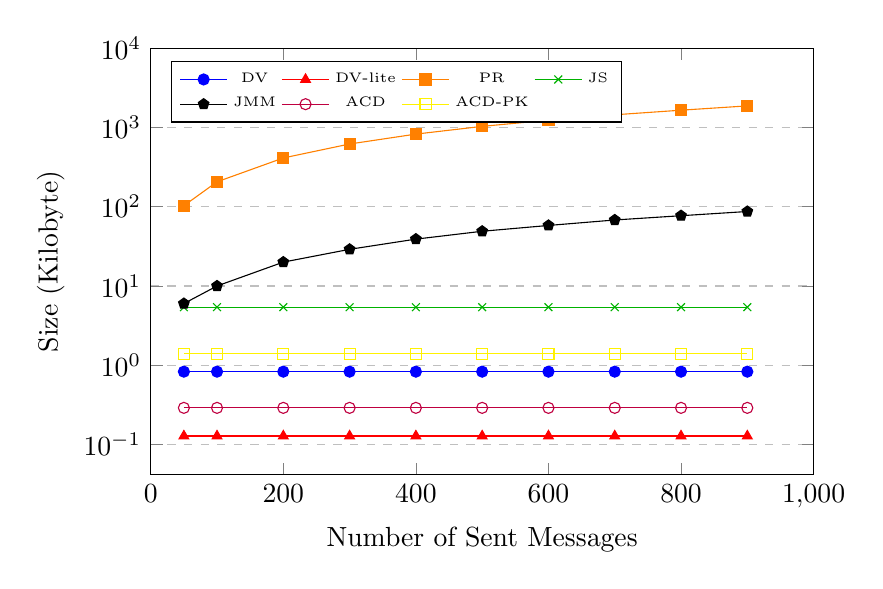
\begin{tikzpicture}[scale=1]
\begin{axis}[
  %ymode=log,
%  legend style={font=\tiny, legend columns=4},
%  scaled ticks=false,
%  xlabel={Number of Sent Messages},
%  ylabel={Size (Kilobyte)},
%  xmin=0, xmax=1000,
%  ymax=200,
%  xtick={0,200,400,600,800,1000},
%  %ytick={0.01,0.1,1,10,100,1000,10000},
%  ytick={0,20,40,60,80,100,120,140,160,180,200},
%  legend pos=north west,
%  ymajorgrids=true,
%  xminorticks=false,
%  yminorticks=false,
%  grid style=dashed,
%  height=7cm,
%  width=10cm,
  ymode=log,
  legend style={font=\tiny, legend columns=4},
  scaled ticks=false,
  xlabel={Number of Sent Messages},
  ylabel={Size (Kilobyte)},
  xmin=0, xmax=1000,
  ymax=10000,
  xtick={0,200,400,600,800,1000},
  ytick={0.001,0.01,0.1,1,10,100,1000,10000},
  %ytick={0,20,40,60,80,100,120,140,160,180,200},
  legend pos=north west,
  ymajorgrids=true,
  xminorticks=false,
  yminorticks=false,
  grid style=dashed,
  height=7cm,
  width=10cm,
]
 
\addplot[color=blue,mark=*]
   coordinates {
  (50,0.83)(100,0.83)(200,0.83)(300,0.83)(400,0.83)(500,0.83)(600,0.83)
  (700,0.83)(800,0.83)(900,0.83)
  };

\addplot[color=red,mark=triangle*]
  coordinates {
  (50,0.128)(100,0.128)(200,0.128)(300,0.128)(400,0.128)(500,0.128)
  (600,0.128)(700,0.128)(800,0.128)(900,0.128)
  };

\addplot[color=orange,mark=square*]
  coordinates {
  (50,103)(100,206)(200,412)(300,618)(400,824)(500,1031)
  (600,1237)(700,1444)(800,1650)(900,1870)
  };


\addplot[color=black!30!green,mark=x]
  coordinates {
  (50,5.4)(100,5.4)(200,5.4)(300,5.4)(400,5.4)(500,5.4)
  (600,5.4)(700,5.4)(800,5.4)(900,5.4)
  };

\addplot[color=black,mark=pentagon*]
  coordinates {
  (50,6)(100,10)(200,20)(300,29)(400,39)(500,49)
  (600,58)(700,68)(800,77)(900,87)
  };

\addplot[color=purple,mark=o]
  coordinates {
  (50,0.29)(100,0.29)(200,0.29)(300,0.29)(400,0.29)(500,0.29)
  (600,0.29)(700,0.29)(800,0.29)(900,0.29)
  };

\addplot[color=yellow,mark=square]
  coordinates {
  (50,1.4)(100,1.4)(200,1.4)(300,1.4)(400,1.4)(500,1.4)
  (600,1.4)(700,1.4)(800,1.4)(900,1.4)
  };


  \legend{DV,DV-lite,PR,JS,JMM,ACD,ACD-PK}
 
\end{axis}
\end{tikzpicture} 
  \caption{State Size Benchmark Alternating Traffic}
  \label{fig:state-size-alt}
\end{figure}

In alternating traffic there is no accumulation of keys,
hence the constant state sizes for the JS, DV and ACD protocols.
Both the PT and JMM protocols however require that the
entire message transcript is kept in the user states
resulting in a linear growth of the states.

\subsection{(Deferred) Unidirectional Traffic}
\label{sec:unid-traff-2}

\begin{figure}[H]
  \centering
  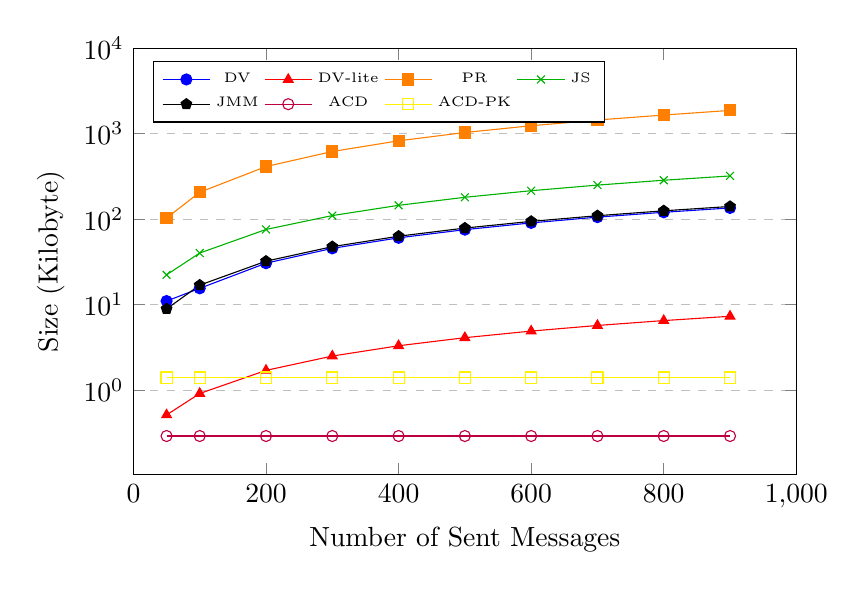
\begin{tikzpicture}[scale=1]
\begin{axis}[
  %ymode=log,
%  legend style={font=\tiny, legend columns=4},
%  scaled ticks=false,
%  xlabel={Number of Sent Messages},
%  ylabel={Size (Kilobyte)},
%  xmin=0, xmax=1000,
%  ymax=200,
%  xtick={0,200,400,600,800,1000},
%  %ytick={0.01,0.1,1,10,100,1000,10000},
%  ytick={0,20,40,60,80,100,120,140,160,180,200},
%  legend pos=north west,
%  ymajorgrids=true,
%  xminorticks=false,
%  yminorticks=false,
%  grid style=dashed,
%  height=7cm,
%  width=10cm,
  ymode=log,
  legend style={font=\tiny, legend columns=4},
  scaled ticks=false,
  xlabel={Number of Sent Messages},
  ylabel={Size (Kilobyte)},
  xmin=0, xmax=1000,
  ymax=10000,
  xtick={0,200,400,600,800,1000},
  ytick={0.001,0.01,0.1,1,10,100,1000,10000},
  %ytick={0,20,40,60,80,100,120,140,160,180,200},
  legend pos=north west,
  ymajorgrids=true,
  xminorticks=false,
  yminorticks=false,
  grid style=dashed,
  height=7cm,
  width=10cm,
]
 
\addplot[color=blue,mark=*]
   coordinates {
  (50,11.0)(100,15.5)(200,30.5)(300,45.5)(400,60.4)(500,75.3)(600,90.3)
  (700,105.5)(800,120.2)(900,135.1)
  };

\addplot[color=red,mark=triangle*]
  coordinates {
  (50,0.512)(100,0.912)(200,1.7)(300,2.5)(400,3.3)(500,4.1)
  (600,4.9)(700,5.7)(800,6.5)(900,7.3)
  };

\addplot[color=orange,mark=square*]
  coordinates {
  (50,103)(100,206)(200,412)(300,618)(400,824)(500,1031)
  (600,1237)(700,1444)(800,1650)(900,1870)
  };


\addplot[color=black!30!green,mark=x]
  coordinates {
  (50,22.3)(100,40.1)(200,75.7)(300,110)(400,145)(500,180)
  (600,215)(700,250)(800,285)(900,320)
  };

\addplot[color=black,mark=pentagon*]
  coordinates {
  (50,8.9)(100,16.9)(200,32.2)(300,47.6)(400,63.1)(500,78.6)
  (600,94.1)(700,109.6)(800,125.1)(900,140.6)
  };

\addplot[color=purple,mark=o]
  coordinates {
  (50,0.29)(100,0.29)(200,0.29)(300,0.29)(400,0.29)(500,0.29)
  (600,0.29)(700,0.29)(800,0.29)(900,0.29)
  };

\addplot[color=yellow,mark=square]
  coordinates {
  (50,1.4)(100,1.4)(200,1.4)(300,1.4)(400,1.4)(500,1.4)
  (600,1.4)(700,1.4)(800,1.4)(900,1.4)
  };


  \legend{DV,DV-lite,PR,JS,JMM,ACD,ACD-PK}
 
\end{axis}
\end{tikzpicture} 
  \caption{State Size Benchmark Unidirectional Traffic}
  \label{fig:state-size-uni}
\end{figure}

In all protocols, except ACD, we now have the accumulation
of keys that let the states grow linearly. It is then not
hard to see that we get the same results for deferred
unidirectional traffic so the corresponding figure
is omitted.

\section{Installation}
\label{sec:installation}

The code for all the protocols in located in a
publicly available repository
\footnote{\url{https://github.com/qantik/ratcheted/}} and
can be freely altered and run. Currently, only Linux
or MacOS are supported platforms.

\subsection{Requirements}
\label{sec:requirements}

Only a handful of auxiliary software is required to
be able to run the program.
\begin{enumerate}
\item \textbf{Go.} A working installation of the
  Go programming language of the latest version, 1.11 as of
  January 2019. Go is freely available through any
  system package manager.
\item \textbf{Dep.} Dep is the Go dependency
  manager~\footnote{\url{https://golang.github.io/dep/}}. Dep
  is required to download all the dependencies used
  in the codebase.
\item \textbf{PBC.} The Stanford Pairing-Based Cryptography library
  for the HIBE constructions. It should be available through any
  system package manager, otherwise it can be installed
  manually~\footnote{\url{https://crypto.stanford.edu/pbc/}}.
\end{enumerate}
Please, see the repository \texttt{README} file for a
step-by-step manual for downloading and setting
up the codebase.

\subsection{Repository Structure}
\label{sec:repository-structure}

The codebase is divided, as it is Go practice, into several
packages. The \texttt{PR}, \texttt{JS}, \texttt{DV},
\texttt{JMM} and \texttt{ACD} packages contain
the code of the protocols together with the test-suite
and the benchmarks. The \texttt{primitives} packages
contains the code for the hand-coded primitives
like the Gentry-Silverberg HIBE or the Bellare
et al.~forward-secure signature scheme. Furthermore,
there is the \texttt{report} package containing
the \LaTeX{} source of this very report and the
\texttt{slides} package with the \LaTeX{} source
for the slides accompanying the report. Last but
not least the entire documentation of the
codebase is also available
online~\footnote{\url{https://godoc.org/github.com/qantik/ratcheted}}.

\chapter{Conclusion}
\label{chap:conclusion}

\section{Future Work}
\label{sec:future-work}

Although the benchmarks already reveal a lot regarding the feasibility
of the protocols, they still are rather constructed. It would be thus
interesting to see how the protocols behave in a real-world context
especially in combination with some lower level communication
protocol. One could even envision a fork of the Signal Android
application that replaces the double ratchet with the protocols
treated in this project \footnote{\url{https://github.com/signalapp/Signal-Android}}.
Although Go is already a fast compiled language it does
not reach the efficiency of a C/C++ program so additional performance
gains are within reach. The protocols themselves offer
the possibility of further tinkering. Can some of them be made
more efficient by changing the algorithms or replacing
heavy primitives with lighter alternatives without compromising
the security guarantees? Finally, the protocols are prime starting
points for the construction of new ratcheting protocols.

\section{Gained Knowledge}
\label{sec:gained-knowledge}

The project familiarized me with the theoretical and practical aspects
of ratcheting protocols.  It deepened my understanding of the standard
tools, like games and reduction, used to evaluate and proof the
security guarantees of a protocol. It was an enlightening experience
to see how the composition of many components eventually leads to
advanced multifaceted protocols that can be put to the test in an
implementation. Since none of the protocols were alike often deploying
widely different primitives it offered me the possibility to get to
know some more obscure primitives likes HIBE schemes or forward-secure
signatures. On a more practical note I could further solidify my
programming skills with the implementation, debugging and benchmarking
of the protocols that were more often than not of rather complex
nature culminating in several thousand lines of code. It was further
my first time I could actually roll out my own crypto implementation
motivated by the lack of existing implementation like the
pairing-based HIBE schemes. The schedule especially during the first
weeks of the semester was often tight and some results had to be
obtained on short notice, all of which helped me broaden my ability to
digest complex and long papers and concepts in small time intervals, which
I think is a very valuable skill that also finds its applications outside of
school. It was then especially motivating to see the obtained result
become part of further work. I am also very grateful for the excellent
support by my supervisors that made this project thoroughly enjoyable
experience.

\bibliographystyle{plainurl}
\bibliography{bibliography}

\addcontentsline{toc}{chapter}{\listfigurename}
\listoffigures

\end{document}
